% !TEX encoding = UTF-8 Unicode
\documentclass[a4paper]{article}


\usepackage{color}
\usepackage{url}
\usepackage[T2A]{fontenc} % enable Cyrillic fonts
\usepackage[utf8]{inputenc} % make weird characters work
\usepackage{dirtytalk}
\usepackage{graphicx}
\usepackage{here} 


\usepackage[english,serbian]{babel}
%\usepackage[english,serbianc]{babel} %ukljuciti babel sa ovim opcijama, umesto gornjim, ukoliko se koristi cirilica

\usepackage[unicode]{hyperref}
\hypersetup{colorlinks,citecolor=green,filecolor=green,linkcolor=blue,urlcolor=blue}

\usepackage{listings}

%\newtheorem{primer}{Пример}[section] %ćirilični primer
\newtheorem{primer}{Primer}[section]

\definecolor{mygreen}{rgb}{0,0.6,0}
\definecolor{mygray}{rgb}{0.5,0.5,0.5}
\definecolor{mymauve}{rgb}{0.58,0,0.82}

\lstset{ 
  backgroundcolor=\color{white},   % choose the background color; you must add \usepackage{color} or \usepackage{xcolor}; should come as last argument
  basicstyle=\scriptsize\ttfamily,        % the size of the fonts that are used for the code
  breakatwhitespace=false,         % sets if automatic breaks should only happen at whitespace
  breaklines=true,                 % sets automatic line breaking
  captionpos=b,                    % sets the caption-position to bottom
  commentstyle=\color{mygreen},    % comment style
  deletekeywords={...},            % if you want to delete keywords from the given language
  escapeinside={\%*}{*)},          % if you want to add LaTeX within your code
  extendedchars=true,              % lets you use non-ASCII characters; for 8-bits encodings only, does not work with UTF-8
  firstnumber=1000,                % start line enumeration with line 1000
  frame=single,	                   % adds a frame around the code
  keepspaces=true,                 % keeps spaces in text, useful for keeping indentation of code (possibly needs columns=flexible)
  keywordstyle=\color{blue},       % keyword style
  language=Python,                 % the language of the code
  morekeywords={*,...},            % if you want to add more keywords to the set
  numbers=left,                    % where to put the line-numbers; possible values are (none, left, right)
  numbersep=5pt,                   % how far the line-numbers are from the code
  numberstyle=\tiny\color{mygray}, % the style that is used for the line-numbers
  rulecolor=\color{black},         % if not set, the frame-color may be changed on line-breaks within not-black text (e.g. comments (green here))
  showspaces=false,                % show spaces everywhere adding particular underscores; it overrides 'showstringspaces'
  showstringspaces=false,          % underline spaces within strings only
  showtabs=false,                  % show tabs within strings adding particular underscores
  stepnumber=2,                    % the step between two line-numbers. If it's 1, each line will be numbered
  stringstyle=\color{mymauve},     % string literal style
  tabsize=2,	                   % sets default tabsize to 2 spaces
  title=\lstname                   % show the filename of files included with \lstinputlisting; also try caption instead of title
}

\begin{document}

\title{Informacioni sistem za firmu Duma Group\\ \small{Seminarski rad u okviru kursa\\Informacioni sistemi\\ Matematički fakultet}}

\author{Miloš Miković, Anđela Križan, Milica Galjak, \\ Veronika Miljaković, Nikoleta Vukajlović}

%\date{9.~april 2015.}

\maketitle

%\abstract{
%Ovde ide abstract
%}
\newpage
\tableofcontents

\newpage

\section{Uvod}

 Sistem je skup delova koji funkcionišu zajedno radi ostvarenja zajedničkog cilja ili svrhe. U domenu informatike i računarstva značajnu ulogu imaju \textbf{Informacioni sistemi}. Internacionalna federacija za obradu podataka (International Federation for Information Processing - IFIP) definiše informacioni sistem na sledeći način: "Informacioni sistem je sistem koji prikuplja, pohranjuje, čuva, obrađuje i isporučuje informacije važne za organizaciju i društvo, tako da budu dostupne i upotrebljive za svakog ko se želi njima koristiti, uključujući poslovodstvo, klijente, zaposlene i ostale. Informacioni sistem aktivni je društveni sistem koji se može, ali i ne mora, koristiti      informacionom tehnologijom." 
    
 Predmet ovog rada je razvijanje informacionog sistema za firmu Duma Group iz Novog Sada. Izrađen je kao grupni projekat u okviru predmeta Informacioni sistemi, koji se sluša na prvoj godini master studija Matematičkog fakulteta u Beogradu.

\section{Analiza sistema}

Firma Duma Group se bavi organizovanjem proslava i događaja. U firminoj ponudi nalaze se brojne usluge čiji je cilj da obezbedi korisnicima sve ono što im je za njihove događaje potrebno. Među ovim uslugama su ketering, fotograf i prenosivi bar.

Prilikom formiranja ovog informacionog sistema poseban akcenat ćemo staviti na mađusobnu komunikaciju zaposlenih u firmi, kao i na komunikaciju sa klijentima, jer je to od velikog značaja za unapređenje firme.
    
Klijenti mogu da naprave svoj nalog na sajtu i svojom prijavom dobija mogućnost naručivanja određenih usluga. On popunjava potrebne informacije vezane za događaj, a zatim menadžer organizuje osoblje po klijentovoj narudžbini. Ukoliko se klijent opredeli za usluge keteringa ili prenosivog bara, osoblje ima zadatak da pripremi sadržaj koji je klijent tražio i zadovolji sve njegove potrebe. Dostavljači nakon toga dostavljaju sav potreban sadržaj.
Ukoliko se klijent opredeli za fotografiju, fotografi pripremaju potrebnu opremu za događaj i na dan događaja odlaze na mesto održavanja gde fotografišu i snimaju korisnika i njegove goste. Nakon toga sledi izrada fotografija. 
    
Osnovna svrha sistema je da omogući klijentima da njihov događaj izgleda onako kako su zamislili i da mu za njega budu dostupne sve usluge koje su im potrebne. 

%%dijagram konteksta
\newpage
Na slici \ref{fig:Tok} je prikazan dijagram konteksta informacionog sistem.
    
    \begin{figure}[H]
    \centering
    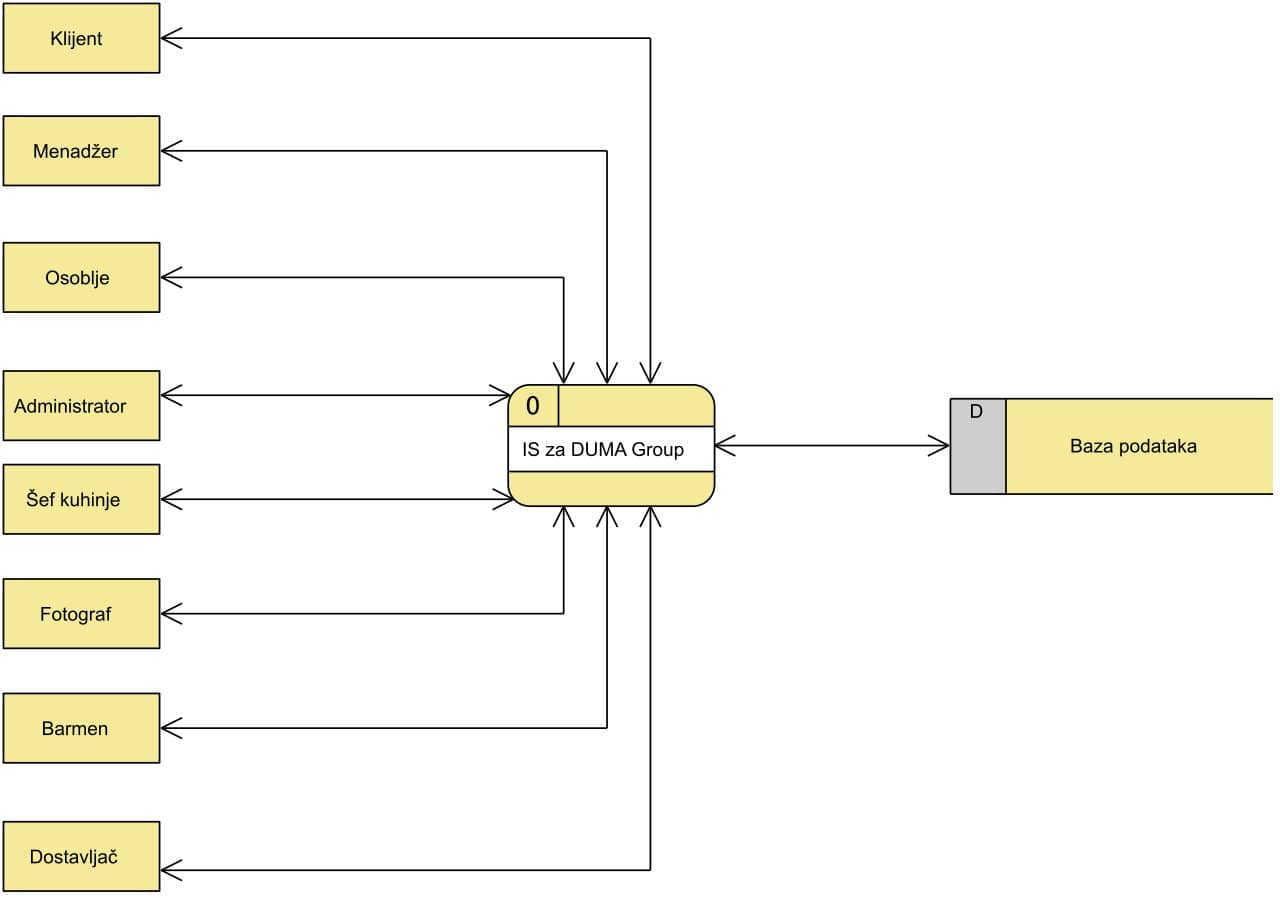
\includegraphics[width=16cm, height=12cm]{Milica/DijagramKonteksta.jpg}
    
    \caption{Dijagram konteksta}
    \label{fig:Tok}
\end{figure}

\newpage
Na slici \ref{fig:Tok} je prikazan dijagram toka podataka nivoa 0.
    
    \begin{figure}[H]
    \centering
    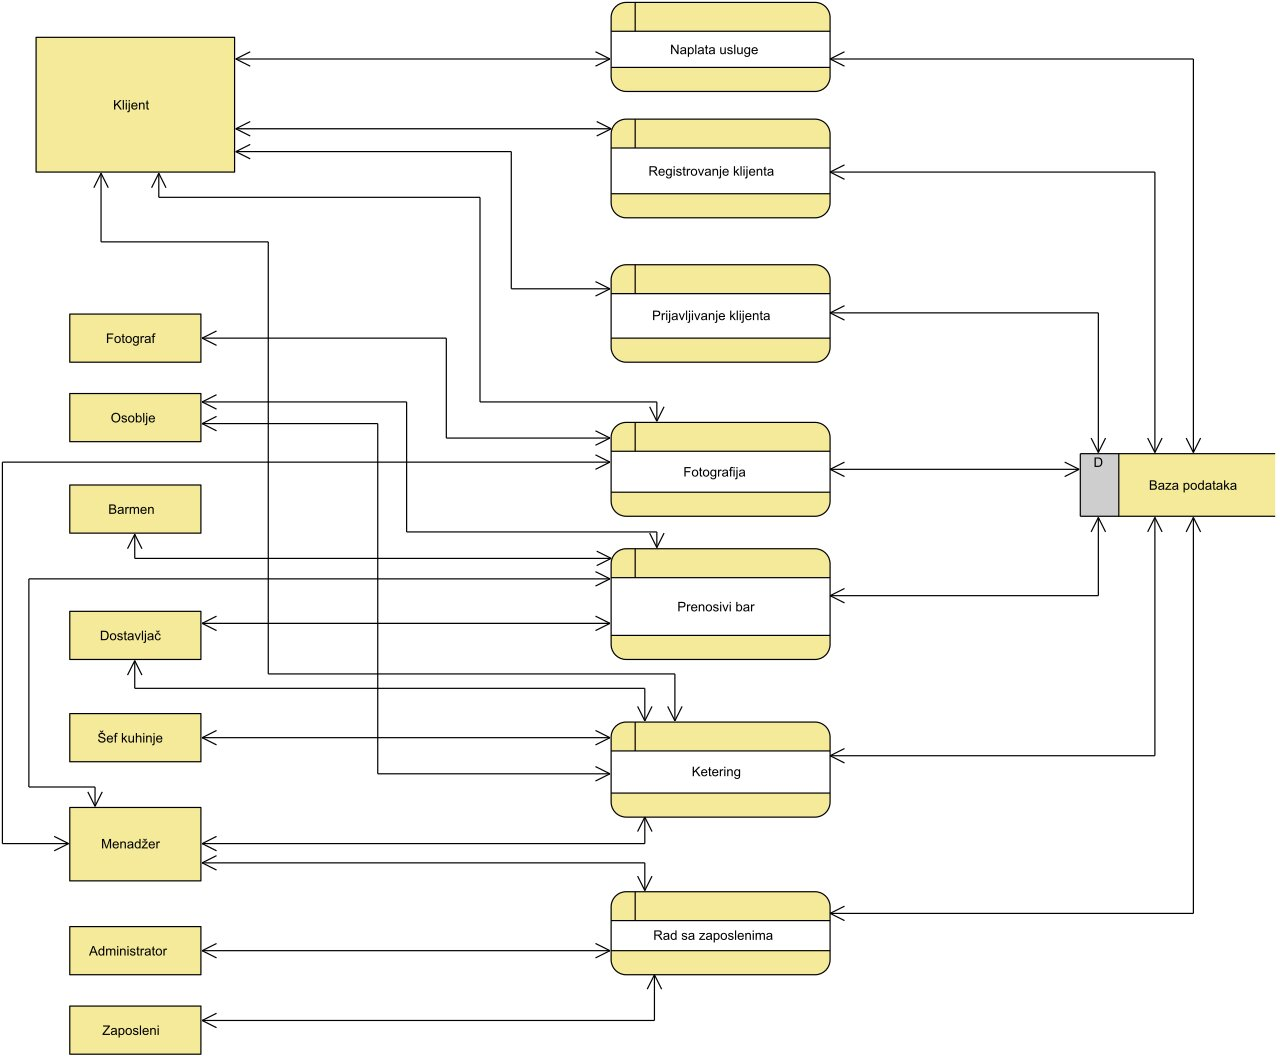
\includegraphics[width=15cm, height=14cm]{Milica/Dijagram_Toka_Podataka.jpg}
    \caption{Dijagram toka podataka nivoa 0}
    \label{fig:Tok}
\end{figure}
    
    \subsection{Učesnici u sistemu}
    
    \begin{enumerate}
        \item Klijenti su svi oni kojima je potrebna usluga koju pruža firma Duma Group. Po završetku usluge vrše uplatu definisanih sredstava preko žiro računa.
        \item Menadžer je osoba koja je zadužena za komunikaciju između klijenata i zaposlenih. Prihvata ponudu i pristupa informacijama za kontaktiranje zaposlenih i klijenata putem informacionog sistema.
        \item Administrator je osoba koja je zadužena da obavi registraciju zaposlenog koji nema kreiran nalog u sistemu, kao i da obriše nalog nakon prekida radnog odnosa sa zaposlenim.
        \item Osoblje su svi oni koji su zaposleni za određeni događaj. Zadatke dobijaju od zaposlenih kao što je menadžer, šef kuhinje...
        \item Šef kuhinje je osoba koja je zadužena da upravlja organizacijom posla u kuhinji. Nadređeni je osoblju u kuhinji i zadužen je za podelu posla u kuhinji. Informacije o samom događaju prima od menadžera.
        \item Fotografi su osobe koje su zadužene za fotografisanje i snimanje gostiju na događaju. Nakon događaja njihov zadatak je da obrade materijal i pripreme finalni proizvod u vidu albuma ili buka. Informacije o događaju i zahtevima klijenta prima od menadžera.
        \item Barmen je osoba koja je zadužena za posluživanje pića gostima i beleženje toga šta je popijeno, u sklopu usluge Prenosivi bar
        \item Dostavljač je osoba koja je zadužena da isporuči poručenu opciju od strane klijenta. Detalje o samoj isporuci dobija putem aplikacije.
    \end{enumerate}
    
    
\section{Slučajevi upotrebe}

% Ovo je moj deo - Miloš

\subsection{Registrovanje i prijavljivanje korisnika}

\begin{figure}[htp]
    \centering
    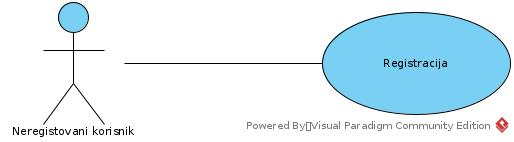
\includegraphics[width=8cm]{Miloš/Miloš_Slučajevi_upotrebe_slike/Slucaj upotrebe _Registrovanje.jpg}
    \caption{Dijagram slučaja upotrebe Registracija korisnika}
    \label{fig:Registracija}
\end{figure}

\subsubsection{Registrovanje klijenta}

\begin{itemize}
    \item Kratak opis:
        \begin{itemize}
            \item Klijent se registruje kako bi mogao da koristi mogućnosti informacionog sistema Duma Group
        \end{itemize}
    \item Učesnici:
        \begin{itemize}
            \item Klijent koji želi da koristi usluge Duma Group sistema
        \end{itemize}
    \item Preduslov:
        \begin{itemize}
            \item Klijent poseduje računar ili pametni telefon i pristup Internetu
            \item Sistem je u funkciji
        \end{itemize}
    \item Postuslov:
        \begin{itemize}
            \item Klijent je registrovan i otvoren mu je nalog za korišćenje sistema
        \end{itemize}
    \item Glavni tok:
        \begin{enumerate}
            \item  Klijent otvara stranicu za registraciju odabirom određenog dugmeta na sajtu sistema
            \item Klijent čita uslove korišćenja sistema i prihvata ih
            \item Klijent popunjava formular unoseći tražene lične podatke. Kada zavši popunjavanje formulara pritiska dugme za registraciju
            \item Sistem obrađuje podatke i vrši validaciju
            \item Sistem kreira privremeni korisnički nalog
            \item Sistem šalje klijentu poruku na e-mail adresu unetu u formularu, postavlja predviđeno vreme za aktivaciju naloga i čeka
            \item Klijent proverava poštu i potvrđuje link za registraciju
            \item Sistem obeležava korisnički nalog kao aktivan i čuva podatke o nalogu
            \item Sistem obaveštava klijenta slanjem poruke na e-mail adresu klijenta da je nalog uspešno kreiran 
        \end{enumerate}
    \item Alternativni tok:
        \begin{itemize}
            \item Korak 2 - klijent odbija uslove korišćenja sistema. Sistem obaveštava korisnika da mora da prihvati date uslove korišćenja, vraća ga na 2. korak glavnog toka i onemogućava dalji tok registracije dok klijent ne prihvati date uslove.
            \item Korak 4 - ukoliko klijent nije uneo ispravne podatke, sistem obaveštava klijenta i proces se nastavlja od 3. koraka glavnog toka
            \item Korak 7 - Ukoliko klijent nije prihvatio aktivacionu poruku u određenom vremenskom periodu, sistem briše nalog i proces se završava.
            \item Korak 7 - Ukoliko klijent nije primio aktivacionu poruku on obaveštava sistem da mu ponovo pošalje poruku i proces se nastavlja od koraka 6. glavnog toka
        \end{itemize}
    \item Dodatne informacije:
        \begin{itemize}
            \item Potrebni podaci za registraciju su korisničko ime, lozinka, potvrda lozinke, broj kreditne kartice, ime, prezime, e-mail naloga, e-mail za povratak naloga ako se desi da je korisnik zaboravi lozinku ili korisničko ime, datum rodjenja korisnika, pol korisnika
            \item Ova registracija predstavlja registraciju klijenata sistema, postoji i registracija zaposlenih koja se vrši odvojeno
        \end{itemize}
\end{itemize}

\begin{figure}[htp]
    \centering
    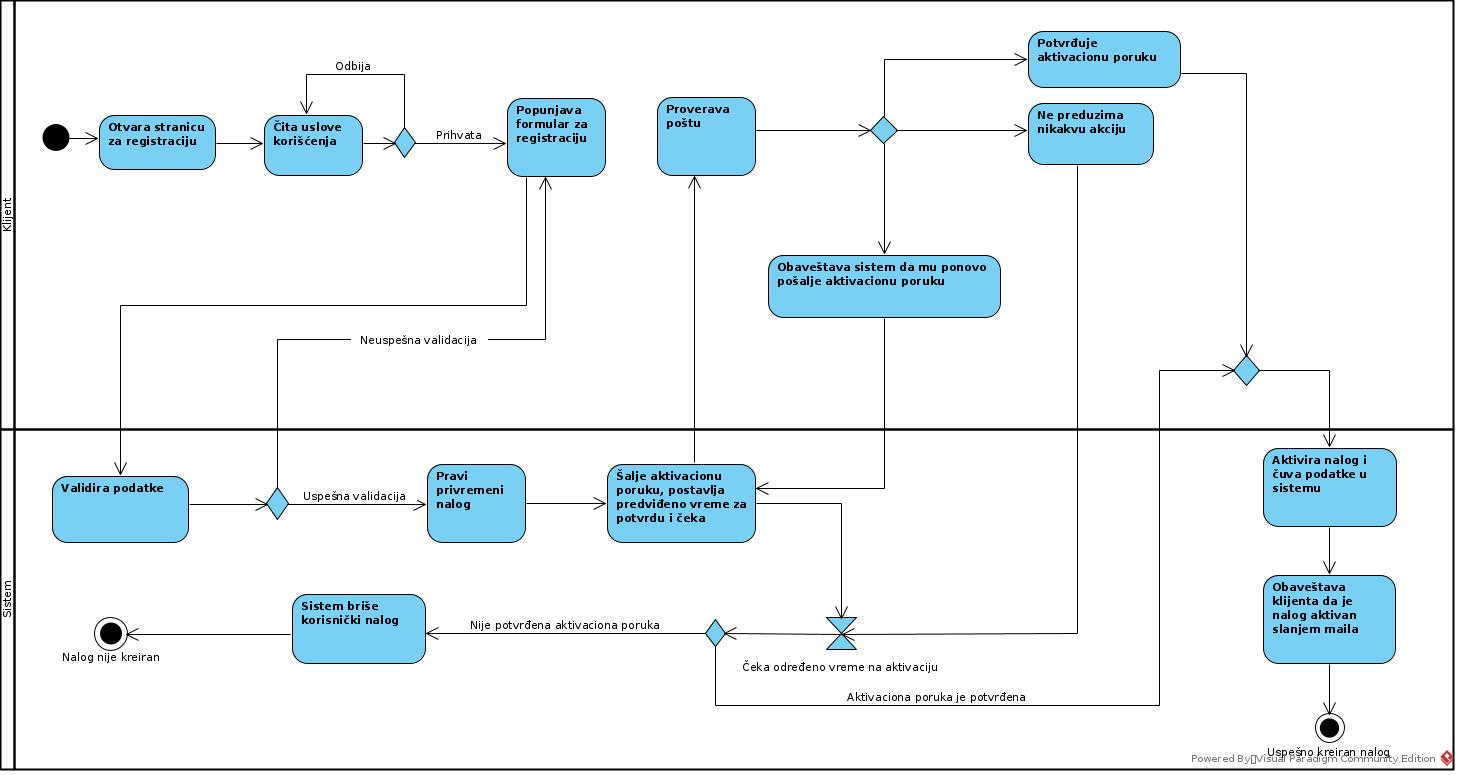
\includegraphics[width=15cm]{Miloš/Miloš_Dijagrami_aktivnosti_slike/Dijagram_aktivnosti_Registrovanje.jpg}
    \caption{Dijagram aktivnosti - Registrovanje korisnika}
    \label{fig:Registracija aktivnost}
\end{figure}


\subsubsection{Prijavljivanje korisnik}

\begin{figure}[htp]
    \centering
    
\includegraphics[width=8cm]{Miloš/Miloš_Slučajevi_upotrebe_slike/Slucaj upotrebe _Prijavljivanje.jpg}
    \caption{Dijagram slučaja upotrebe Prijavljivanje korisnika}
    \label{fig:Prijavljivanje}
\end{figure}

\begin{itemize}
    \item Kratak opis:
        \begin{itemize}
            \item Prethodno registrovani korisnik se prijavljuje na sistem
        \end{itemize}
    \item Učesnici:
        \begin{itemize}
            \item Registrovani korisnik koji želi da se prijavi na sistem
        \end{itemize}
    \item Preduslov:
        \begin{itemize}
            \item Korisnik mora biti registrovan u sistemu da bi se uspešno prijavio
            \item Korisnik poseduje računar ili pametni telefon i pristup Internetu
            \item Sistem je u funkciji
        \end{itemize}
    \item Postuslov:
        \begin{itemize}
            \item Korisnik je prijavljen i može da koristi funkcionalnosti koje sistem pruža
        \end{itemize}
    \item Glavni tok:
        \begin{enumerate}
            %Možda da dodate početni korak da se otvara odgovarajuća stranica za
            %prijavu na sistem. Drugi korak može da se podeli na dva koraka. Sistem
            %proverava podatke i sistem prosleđuje korisnika dalje.
            \item Korisnik otvara stranicu za prijavljivanje
            \item Korisnik unosi svoje korisničko ime i šifru koju je koristio pri registraciji
            \item Sistem validira podatke
            \item Sistem sprovodi korisnika ka interfejsu aplikacije
        \end{enumerate}
    \item Alternativni tok:
        \begin{itemize}
            \item Korak 1 - Ukoliko korisnik ne može da se seti podataka za prijavljivanje obaveštava sistem da mu pošalje mail za oporavak. Sistem šalje mail korisniku, korisnik proverava mail i menja podatke u skladu sa instrukcijama koje je dobio u mailu. Sistem čuva izmene koje je korisnik napravio a proces se nastavlja od 1. koraka glavnog toka.
            \item Korak 3 - Ukoliko korisnički podaci nisu ispravni, sistem obaveštava korisnika o grešci i postavlja brojač neuspešnih pokušaja.
            Ako je brojač prethodno postavljen, njegova vrednost se uvećava za jedan. Proces se nastavlja od 2. koraka glavnog toka.
            \item Korak 3 - Ukoliko sistem određen broj puta ne uspe da validira korisničke podatke postavlja zabranu prijavljivanja za tog korisnika na određeni vremenski period. Nakon isteka zabrane izvršavanje se nastavlja od 2. koraka glavnog toka.
        \end{itemize}
    \item Dodatne informacije:
        \begin{itemize}
            \item Zabrana prijavljivanja nakon nekoliko neuspešnih pokušaja postoji radi zaštite podataka i informacija sistema od eventualnih napada.
            \item Prijavljivanje se vrši na isti način i za klijente i za zaposlene u Duma Group preduzeću
        \end{itemize}
\end{itemize}


\begin{figure}[htp]
    \centering
    
\includegraphics[width=15cm]{Miloš/Miloš_Dijagrami_aktivnosti_slike/Dijagram_aktivnosti_Prijavljivanje.jpg}
    \caption{Dijagram aktivnosti - Prijavljivanje korisnika}
    \label{fig:Prijavljivanje aktivnost}
\end{figure}

%Ovo je moj deo - Nina


\subsection{Rad sa zaposlenima}

\begin{figure}[H]
    \centering
    \includegraphics[width=7cm, height=5cm]{Nina/SlucajUpotrebeRadSaZaposlenima.jpg}
    \caption{Dijagram slučaja upotrebe Rad sa zaposlenima}
    \label{fig:RegistracijaZ}
\end{figure}

\subsubsection{Registracija zaposlenog}

\begin{itemize}
    \item Kratak opis: 
    \begin{itemize}
        \item Administrator registruje zaposlenog koji nema otvoren nalog. Sistem izvršava validaciju i vraća potvrdu o registraciji, ukoliko je uspešna.
    \end{itemize}
    \item Učesnici:
        \begin{itemize}
        \item Administrator
    \end{itemize}
    \item Preduslovi:
        \begin{itemize}
            \item Zaposleni nema kreiran nalog.
            \item Zaposleni je predao validan obrazac sa potrebnim podacima za registraciju.
            \item Sistem je u funkciji.
        \end{itemize}
    \item Postuslovi:
        \begin{itemize}
            \item Zaposleni je registrovan i dobija informacije kako da koristi sistem.
        \end{itemize}
    \item Glavni tok:
        \begin{enumerate}
            \item Administrator popunjava formular sa podacima koje je dobio.
            \item Administrator bira poziciju zaposlenog.
            \item Sistem šalje obaveštenje administratoru da potvrdi unos.
            \item Administrator potvrđuje podatke klikom na dugme.
            \item Sistem obaveštava administratora da je uspešno registrovan nalog.
            \item Administrator šalje zaposlenom uputstvo za korišćenje sistema.
        \end{enumerate}
\end{itemize}

\begin{figure}[H]
    \centering
    \includegraphics[width=10cm, height=6cm]{Nina/DijagramAktivnostiRegistracijaZaposlenog.jpg}
    \caption{Dijagram aktivnosti registracije zaposlenog}
    \label{fig:RegistracijaZ}
\end{figure}


\subsubsection{Brisanje naloga zaposlenog}

\begin{itemize}
    \item Kratak opis: 
    \begin{itemize}
        \item Briše se nalog zaposlenog sa kojim je prekinut radni odnos.
    \end{itemize}
    \item Učesnici:
        \begin{itemize}
        \item Menadžer za ketering/fotografiju/prenosivi bar
        \item Administrator
    \end{itemize}
    \item Preduslovi:
        \begin{itemize}
            \item Sa zaposlenim je prekinut radni odnos.
            \item Sistem je u funkciji.
        \end{itemize}
    \item Postuslovi:
        \begin{itemize}
            \item Nalog je obrisan.
        \end{itemize}
    \item Glavni tok:
        \begin{enumerate}
            \item Menadžer šalje zahtev administratoru da obriše nalog.
            \item Administrator pokreće postupak brisanja naloga zaposlenog klikom na dugme za brisanje.
            \item Administrator popunjava informacije o tome da li je zaposleni svojevoljno dao otkaz ili ne.
            \item Administrator potvrđuje brisanje.
            \item Sistem potvrđuje nalog kao obrisan.
        \end{enumerate}
\end{itemize}

\begin{figure}[H]
    \centering
    \includegraphics[width=12cm, height=7cm]{Nina/DijagramAktivnostiBrisanjeNaloga.jpg}
    \caption{Dijagram aktivnosti brisanja naloga}
    \label{fig:RegistracijaZ}
\end{figure}


%Ovo je moj deo - Veronika


\subsection{Prenosivi bar}

\begin{figure}[H]
    \centering
    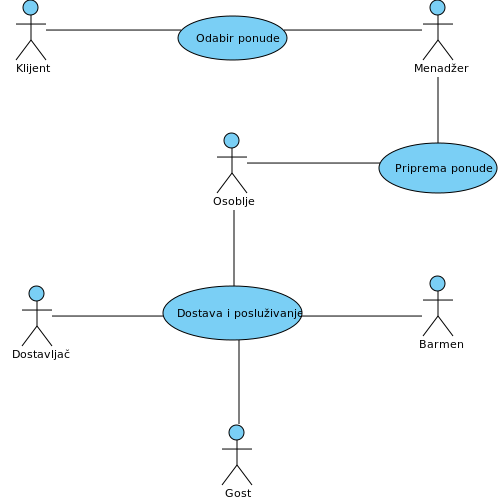
\includegraphics[width=8cm]{Veronika/Dijagram slucaja upotrebe _ Prenosivi bar.png}
    \caption{Dijagram slučaja upotrebe Prenosivi bar}
    \label{fig:PrenosiviBar}
\end{figure}

\subsubsection{Odabir ponude}

\begin{itemize}
    \item Kratak opis:
        \begin{itemize}
            \item Klijent bira odgovarajuću ponudu u skladu sa događajem za koji mu je usluga potrebna
        \end{itemize}
    \item Učesnici:
        \begin{itemize}
            \item Klijent
            \item Menadžer 
        \end{itemize}
    \item Preduslov:
        \begin{itemize}
            \item Klijent se prijavio u sistem
		    \item Na raspolaganju je spisak ponuda sa pratećim informacijama
        \end{itemize}
    \item Postuslov:
        \begin{itemize}
            \item Klijent je odabrao odgovarajuću ponudu
            \item Menadžer je prihvatio odabir i zabeležio potrebne detalje u sistem
        \end{itemize}
    \item Glavni tok:
        \begin{enumerate}
          \item  Klijent se klikom na dugme opredeljuje za uslugu ''Prenosivi bar''.
        \item Klijent bira datum, mesto i vreme početka događaja za koji naručuje ovu uslugu.
        \item Klijent bira sadržaj koji želi iz ponude i svaki odabir se beleži u sistem.
        \item Klijent potvrđuje izabranu porudžbinu.
        \item Menadžeru stiže obaveštenje od aplikacije da ima novu porudžbinu prenosivog bara.
        \item Menadžer prihvata porudžbinu klijenta.
        \item Sistem formira račun za klijenta na koji se dodaju cene prenosivog bara i dekoracije. Cene pića dodaju se naknadno jer klijent plaća samo ono što je na događaju popijeno.
        \end{enumerate}
        \item Alternativni tok:
        \begin{itemize}
            \item Korak 5 - Sadržaj koji je klijent odabrao nije dostupan. U tom slučaju menadžer zamoli klijenta da odabere nešto drugo iz ponude i uputi ga na ponudu koja je slična onoj koju je tražio. Nakon toga klijent ponovo bira sadržaj za svoj događaj.
        \end{itemize}    
    \end{itemize}


\begin{figure}[H]
    \centering
    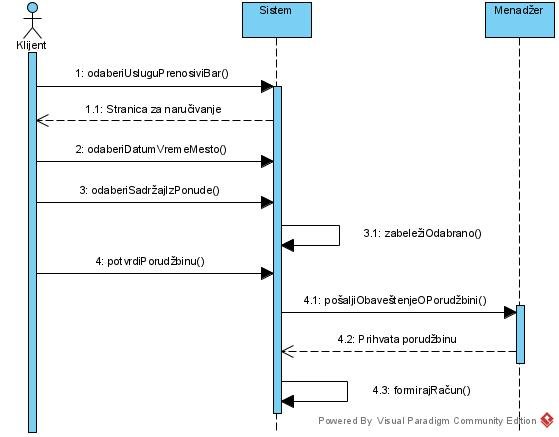
\includegraphics[width=12cm]{Veronika/DijagramSekvence_OdabirPonude.jpg}
    \caption{Dijagram sekvence - Odabir ponude}
    \label{fig:PrenosiviBar}
\end{figure}


\subsubsection{Priprema ponude}

\begin{itemize}
    \item Kratak opis:
        \begin{itemize}
            \item Menadžer prenosi ponudu osoblju koje nakon toga priprema ono što je zahtevano
        \end{itemize}
    \item Učesnici:
        \begin{itemize}
            \item Menadžer 
            \item Osoblje
        \end{itemize}
    \item Preduslov:
        \begin{itemize}
            \item Klijent je odabrao svoju ponudu
		    \item Menadžer je zabeležio ponudu u sistemu
        \end{itemize}
    \item Postuslov:
        \begin{itemize}
            \item Ponuda je pripremljena i spakovana za dostavu
        \end{itemize}
    \item Glavni tok:
        \begin{enumerate}
           \item Menadžer preko sistema šalje izabranu ponudu osoblju tako što odabere u sistemu sve one koji trebaju biti angažovani na događaju i na njihove naloge pošalje koja su im zaduženja
		   \item Osoblje preko svojih naloga preuzima detalje o ponudi
	       \item Osoblje priprema neophodne flaše pića, prenosivi bar i dekoraciju
	       \item Osoblje pakuje sav pripremljeni sadržaj u prevozno sredstvo tako da bezbedno stigne na dogovorenu lokaciju
	       \item Osoblje beleži u sistemu da je sve spremno za dostavu
	       \item Sistem šalje obaveštenje dostavljaču da dostava može da počne
        \end{enumerate}
\end{itemize}

\begin{figure}[H]
    \centering
    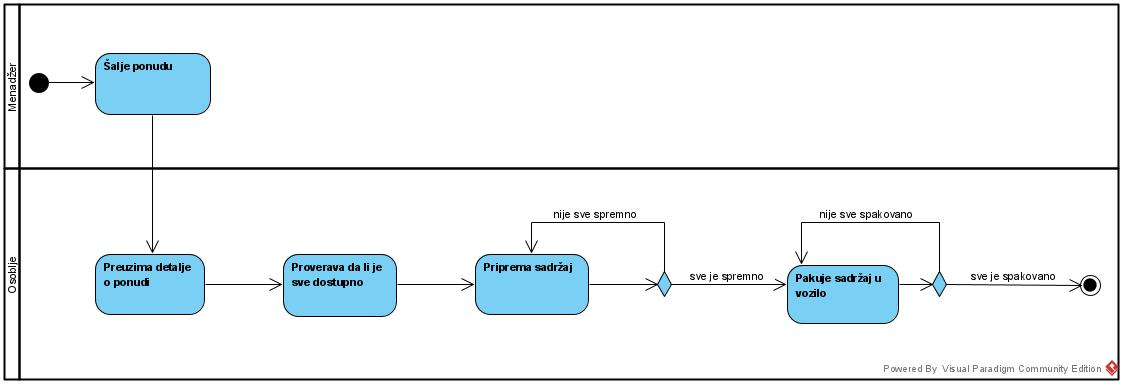
\includegraphics[width=16cm]{Veronika/Dijagram aktivnosti 2 PB.jpg}
    \caption{Dijagram aktivnosti - Priprema ponude}
    \label{fig:PrenosiviBar}
\end{figure}


\subsubsection{Dostava i posluživanje}

\begin{itemize}
    \item Kratak opis:
        \begin{itemize}
            \item Ponuda je dovezena na potrebnu lokaciju i spremna za posluživanje gostiju koje obavlja barmen
        \end{itemize}
    \item Učesnici:
        \begin{itemize}
            \item Dostavljač
            \item Osoblje
            \item Gosti
            \item Barmen 
        \end{itemize}
    \item Preduslov:
        \begin{itemize}
		    \item Dostavljač je na raspolaganju
		     \item Dostavljač je dobio obaveštenje od sistema da dostava može da počne
		    \item Barmen je dobio detalje o mestu i vremenu održavanja događaja
        \end{itemize}
    \item Postuslov:
        \begin{itemize}
            \item Svi gosti su usluženi na odgovarajući način
            \item Na račun su dodate cene popijenih pića
        \end{itemize}
    \item Glavni tok:
        \begin{enumerate}
            \item Dostavljač preuzima informaciju iz sistema gde treba odvesti porudžbinu i osoblje zaduženo za postavljanje prenosivog bara i dekoracije
           \item Dostavljač odvozi robu i osoblje na dogovorenu adresu sat vremena pre početka događaja 
		    \item Osoblje čita iz sistema kako treba postaviti i dekorisati prenosivi bar 
		    \item Osoblje postavlja i dekoriše prenosivi bar
		    \item Barmen dolazi na odgovarajuću adresu koja mu je poslata preko sistema i priprema se za posao
            \item Barmen iz sistema čita spisak pića koje je klijent naručio i proverava da li mu je dostavljeno sve što je naručeno
           \item Gost dolazi do šanka i naručuje piće od barmena
		   \item Barmen uslužuje gosta i beleži u sistem koje je piće naručeno
		   \item Sistem dodaje cenu tog pića na račun korisnika
        \end{enumerate}
     \item Alternativni tok:
        \begin{itemize}
	      \item	Korak 6 - Piće koje gost traži je u međuvremenu popijeno. U tom slučaju barmen preporučuje gostu neka druga pića koja su dostupna i gost bira jedno od njih.  
	      \end{itemize}
\end{itemize}


\begin{figure}[H]
    \centering
    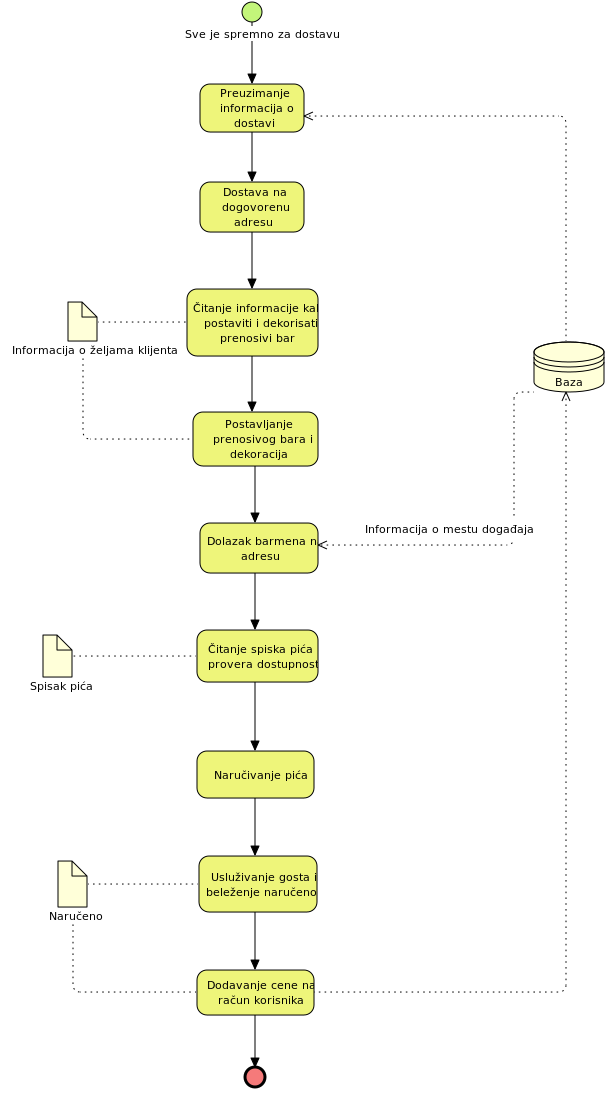
\includegraphics[height=14cm]{Veronika/BPMN Dijagram dostava i posluzivanje PB.png}
    \caption{BPMN dijagram procesa - Dostava i posluživanje}
    \label{fig:PrenosiviBar}
\end{figure}

%%%%%%%%%%%%%%%%%%%%%%%%%%%%%%%%%%%%%%%%%%%%%%%%%%%%%%%%%%%%%%%%%%%%%%%%%%%%%%
% Ovo je moj deo - Andjela

\subsection{Fotografija}

\begin{figure}[H]
    \centering
    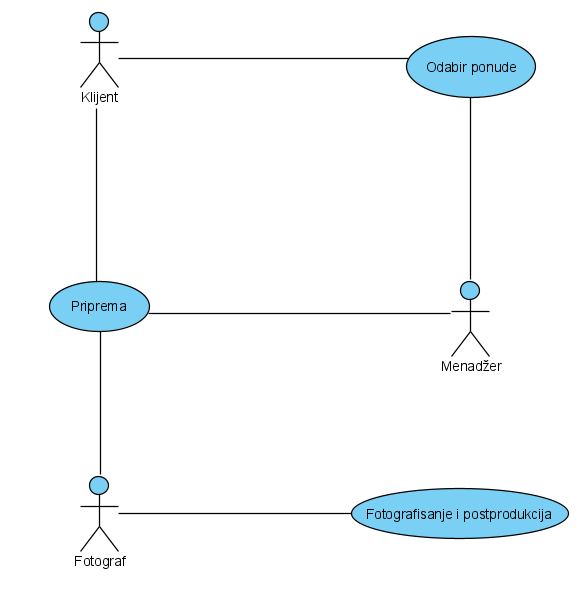
\includegraphics[width=8cm, height=6cm]{Andjela/Dijagram_slucaja_upotrebe_fotografija.png}
    \caption{Dijagram slučaja upotrebe Fotografija}
    \label{fig:PrenosiviBar}
\end{figure}

\subsubsection{Odabir ponude}
\begin{itemize}
    \item Kratak opis: 
    \begin{itemize}
        \item Klijent bira odgovarajuću ponudu u skladu sa događajem za koji mu je usluga potrebna
    \end{itemize}
    \item Učesnici:
        \begin{itemize}
        \item Klijent
        \item Menadžer
    \end{itemize}
    \item Preduslovi:
        \begin{itemize}
            \item Klijent se prijavio na sistem
            \item Na raspolaganju je spisak različitih ponuda sa pratećim slikama i snimcima
        \end{itemize}
    \item Postuslovi:
        \begin{itemize}
            \item Klijent je odabrao odgovarajuću ponudu
            \item Menadžer je prihvatio izbor i zabeležio potrebne detalje u sistem
        \end{itemize}
    \item Glavni tok:
        \begin{enumerate}
            \item Klijent se klikom na dugme opredeljuje za uslugu ''Fotografija''.
            \item Klijent bira datum, mesto, vreme početka događaja, kao i dužinu trajanja.
            \item Klijent bira neku od ponuda na osnovu toga kog je tipa događaj.
            \item Klijent potvrđuje izabranu porudžbinu.
            \item Menadžeru stiže obaveštenje od aplikacije da ima novu porudžbinu za fotografiju.
            \item Klijent se dogovara sa menadžerom oko detalja dogadaja (datum događaja, trajanje, dodatni zahtevi)
            \item Menadžer prihvata porudžbinu klijenta.
            \item Sistem formira račun za klijenta na koji se dodaje cena fotografisanja i izrada finalnog proizvoda(foto album, buk, video snimak...)
        \end{enumerate}
        
    \begin{figure}[H]
    \centering
    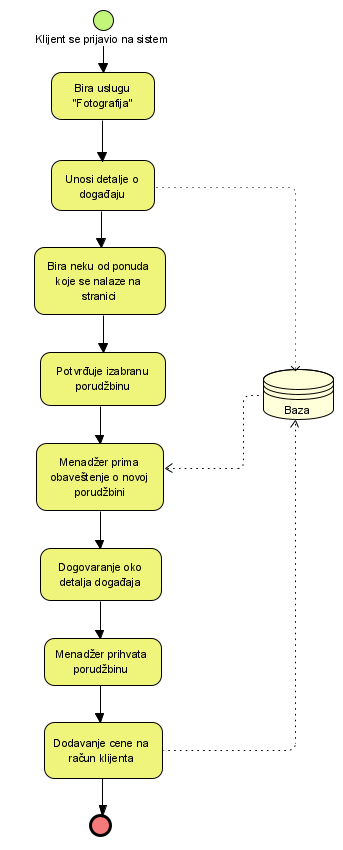
\includegraphics[height=14cm]{Andjela/BPMN_dijagram_fotografija.png}
    \caption{BPMN dijagram procesa - odabir ponude}
    \label{fig:RegistracijaZ}
\end{figure}
        
\end{itemize}

\subsubsection{Priprema}
\begin{itemize}
    \item Kratak opis: 
    \begin{itemize}
        \item Menadžer obaveštava fotografe o rasporedu svečanosti
        %\item Klijent obaveštava o dodatnim zahtevima
    \end{itemize}
    \item Učesnici:
        \begin{itemize}
        %\item Klijent
        \item Fotografi
        \item Menadžer
    \end{itemize}
    \item Preduslovi:
        \begin{itemize}
            \item Klijent je izabrao ponudu
            \item Menadžer je prihvatio ponudu i zabeležio u sistem
        \end{itemize}
    \item Postuslovi:
        \begin{itemize}
            \item Fotografi su pripremili opremu u odnosu na zahtev
        \end{itemize}
    \item Glavni tok:
        \begin{enumerate}
            \item Menadžer preko sistema obaveštava fotografe o rasporedu svečanosti i zahtevima klijenta
            \item Fotografi preuzimaju detalje o zahtevima klijenta
            \item Fotografi pripremaju opremu (rasvetu, kameru, dron...)
            \item Fotografi pripremaju plan fotografisanja u skladu sa zahtevima korisnika
            \item Na dan proslave, fotografi setuju opremu
        \end{enumerate}
        
        \begin{figure}[H]
    \centering
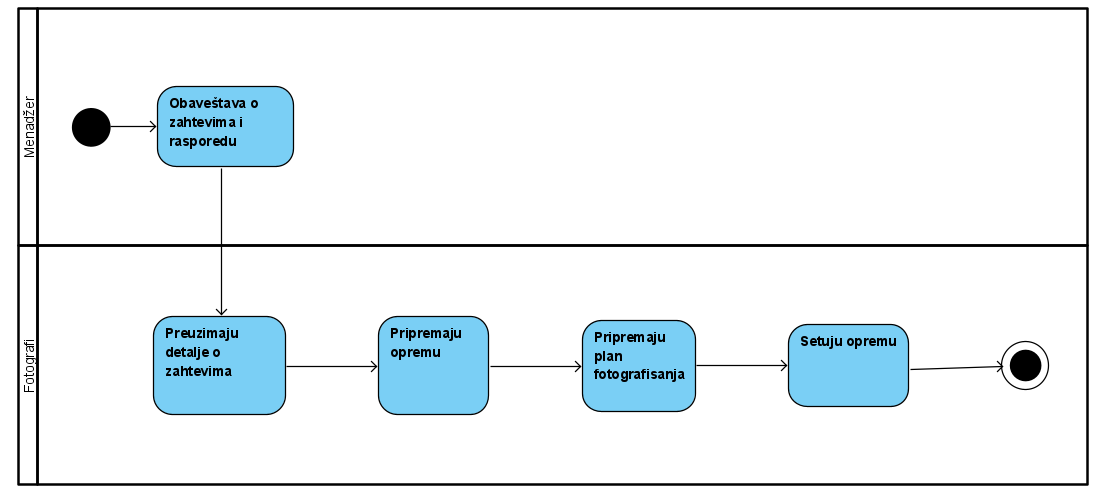
\includegraphics[width=13cm, height=6cm]{Andjela/priprema_fotografija.png}
    \caption{Dijagram aktivnosti pripreme}
    \label{fig:RegistracijaZ}
\end{figure}
        
        
\end{itemize}
\subsubsection{Fotografisanje i postprodukcija}
\begin{itemize}
    \item Kratak opis: 
    \begin{itemize}
        \item Fotografi snimaju i fotografišu događaj, a zatim pregledaju i obrađuju sakupljeni materijal
    \end{itemize}
    \item Učesnici:
        \begin{itemize}
        \item Fotografi
    \end{itemize}
    \item Preduslovi:
        \begin{itemize}
            \item Fotografi su dobili detalje o mestu i vremenu održavanja događaja
            \item Oprema je setovana
            \item Fotografi su na pozicijama i čekaju da svečanost počne
        \end{itemize}
    \item Postuslov:
        \begin{itemize}
            \item Gotov je finalni proizvod
            \item Na račun je dodata cena finalnog proizvoda
            \end{itemize}
    \item Glavni tok:
        \begin{enumerate}
            \item Fotografi dolaze na odgovarajuću adresu koja im je poslata preko sistema
            \item Snimanje i fotografisanje događaja i slavljenika
            \item Pregled sakupljenog materijala
             \item Izrada finalnog proizvoda od sakupljenih fotografija i snimaka. Izbor najuspešnijih kadrova. 
            \item Fotografi beleže u sistem cenu finalnog proizvoda
            \item Sistem dodaje tu cenu na račun korisnika
            
            \textit{Korak 2 se ponavlja za svakog gosta ili slavljenika koji želi da se fotogafiše tokom celog događaja}
            
            \textit{Korak 4 se ponavlja sve dok ne bude završena obrada sirovog materijala i spreman finalni proizvod}
        \end{enumerate}
    \item Alternativni tok:
        \begin{itemize}
            \item Korak 2 - Ukoliko je u pitanju svadba (Post Wedding), dan nakog proslave mladenci i fotografi idu na dogovorenu destinaciju radi fotografisanja. Fotografi naknadno unose tu cenu u sistem
    \end{itemize}
    \item Dodatne informacije:
        \begin{itemize}
            \item Finalni proizvod može biti fotoalbum, fotografije u elektronskoj formi, buk, spot(od 30s do 180s) ili film (kraća i duža verzija)
        \end{itemize}
    
    \begin{figure}[H]
    \centering
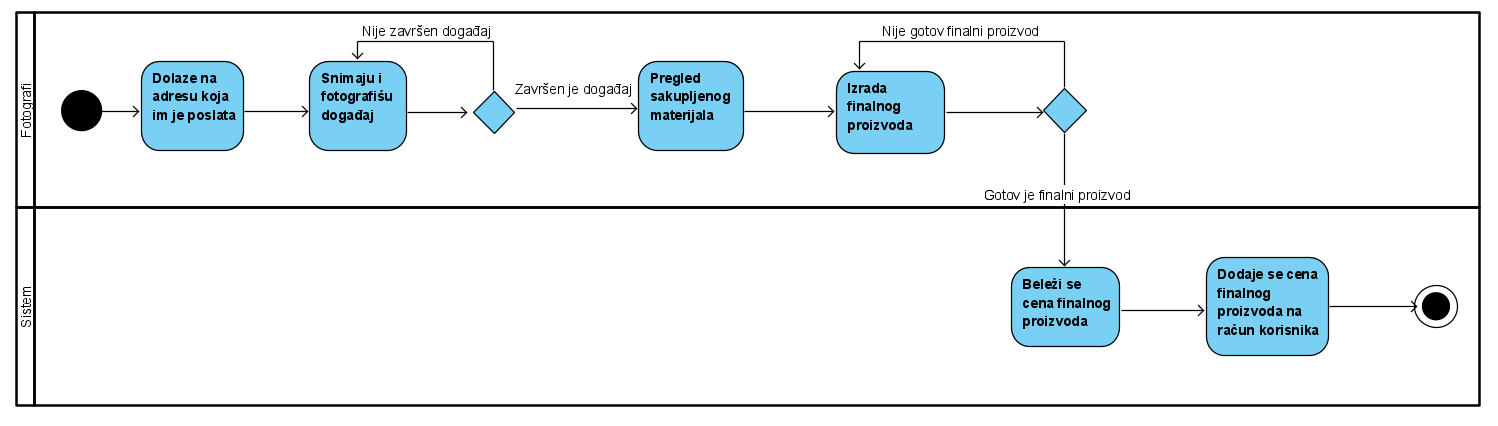
\includegraphics[width=14cm, height=5cm]{Andjela/fotografisanje_i_postprodukcija.png}
    \caption{Dijagram aktivnosti fotografisanja i postprodukcije}
    \label{fig:RegistracijaZ}
\end{figure}
    
        
\end{itemize}

% kraj-Andjela
%%%%%%%%%%%%%%%%%%%%%%%%%%%%%%%%%%%%%%%%%%%%%%%%%%%%%%%%%%%%%%%%%%%%%%%%%%%%%%


%%%%%%%%%%%%%%%%
%pocetak-Milica

\subsection{Ketering}

  
\begin{figure}[H]
\centering
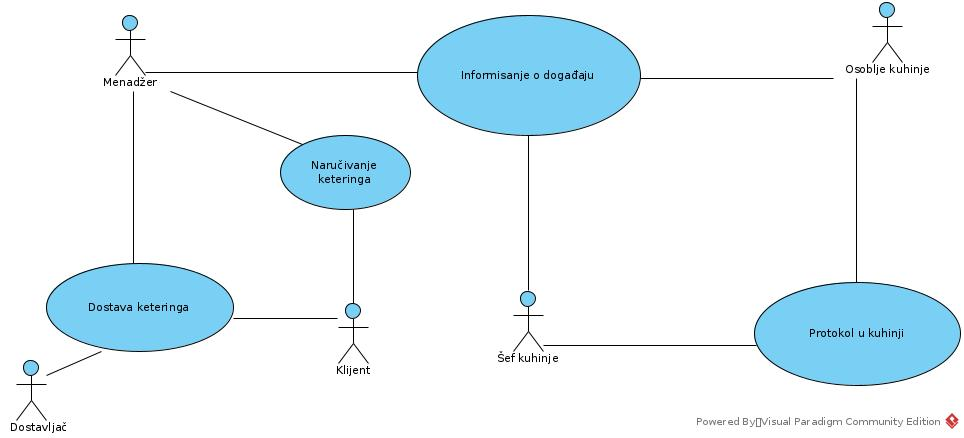
\includegraphics[width=13cm, height=6cm]{Milica/Ketering_Slucaj_upotrebe1.jpg}
\caption{Dijagram slučaja upotrebe Ketering}
\label{fig:Ketering}
\end{figure}

\subsubsection{Naručivanje keteringa i prihvatanje ponude}
\begin{itemize}
    \item Kratak opis:
    \begin{itemize}
 
        \item Klijent putem aplikacije bira željenu ponudu. Menadžer putem aplikacije dobija traženu ponudu, odnosno prihvata je.
    \end{itemize}
    
    
\end{itemize}


  \begin{itemize}
        \item Učesnici:
         \begin{itemize}
        \item Menadžer
    \end{itemize}
          \begin{itemize}
        \item Klijent
    \end{itemize}
    
    \end{itemize}
      \begin{itemize}
        \item Preduslov:
          \begin{itemize}
        \item Klijent je registrovan u sistemu.
       
   \end{itemize}
    
    \end{itemize}
      \begin{itemize}
        \item Postuslov:
          \begin{itemize}
        \item Porudžbina je naručena i prihvaćena od strane menadžera.
    \end{itemize}
    \end{itemize}
      \begin{itemize}
        \item Glavni tok:
          \begin{enumerate}
          
              \item Klijent se uloguje na svoj nalog u aplikaciji, bira kao željenu opciju ketering.
              
              \item Klijent bira datum i vreme početka događaja za koji naručuje ketering i mesto.
          
              \item Nakon toga, klijent bira iz asortimana na aplikaciji željenu ponudu i količinu.
              
              \item Klijent potvrđuje izabranu porudžbinu.
        
              \item Menadžeru stiže obaveštenje od aplikacije da ima novu porudžbinu keteringa.
         
              \item Menadžer prihvata porudžbinu.
      
          \end{enumerate}
    \end{itemize}
    
   
    
\begin{figure}[H]
    \centering
    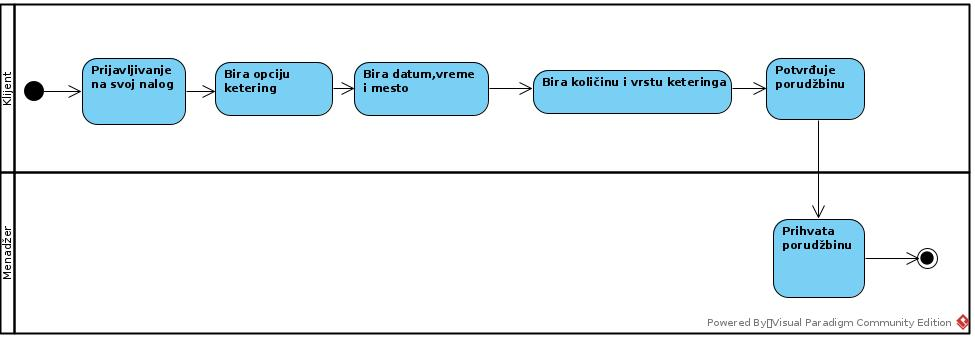
\includegraphics[width=15cm, height=5cm]{Milica/Dijagram_aktivnosti_Narucivanje.jpg}
    \caption{Dijagram aktivnosti Naručivanje keteringa i prihvatanje ponude}
    \label{fig:RegistracijaZ}
\end{figure}

    


\subsubsection{Formiranje tima za događaj}
\begin{itemize}
    \item Kratak opis:
    \begin{itemize}
        \item 
        Menadžer prihvata narudžbinu putem aplikacije. U zavisnosti od datuma za koji je naručena narudžbina, šalje zahtev osoblju koje je raspoloživo tada. Osoblje obeležava u aplikaciji da li želi da radi za zakazani događaj ili ne.
    \end{itemize}
\end{itemize}
  \begin{itemize}
        \item Učesnici:
          \begin{itemize}
        \item Menadžer
    \end{itemize}
      \begin{itemize}
        \item Osoblje
    \end{itemize}
    \begin{itemize}
        \item Šef kuhinje
    \end{itemize}
    \end{itemize}
      \begin{itemize}
        \item Preduslov:
          \begin{itemize}
        \item  Klijent je izabrao željenu ponudu korišćenjem aplikacije.
    \end{itemize}
    
    \end{itemize}
      \begin{itemize}
        \item Postuslov:
          \begin{itemize}
        \item Izabran je tim koji će raditi za zakazani događaj. Šef kuhinje zna koje osoblje je u timu.
    \end{itemize}
    \end{itemize}
      \begin{itemize}
        \item Glavni tok:
          \begin{enumerate}
              \item Menadžer šalje zahtev za potvrdu o radu raspoloživom osoblju. Sa zahtevom šalje i informacije o tipu događaja, detalje o samoj narudžbini keteringa.
        
              \item Svako od osoblja koje je dobilo zahtev vraća odgovor da li želi da radi narudžbinu ili ne.
         
        
              \item Menadžer ima spisak osoblja koje žele da rade događaj.
          
              \item Menadžer šalje spisak osoblja šefu kuhinje.
          \end{enumerate}
    \end{itemize}
      \begin{itemize}
        \item Alternativni tok:
          \begin{itemize}
        \item Korak 4 - Ukoliko nema dovoljno osoblja za zakazani događaj, menadžer stupa u kontakt sa klijentom pomoću podataka koje je klijent ostavio na svom nalogu na aplikaciji, obaveštava ga o tome i izlaže mu druge opcije kao što su promena termina događaja, manja količina poručene hrane...Ukoliko klijent prihvati druge opcije, menadžer ponovo sastavlja tim u skladu sa klijentovom željom da li želi drugi datum ili drugu porudžbinu. Proces se nastavlja u koraku 4.
    \end{itemize}
    \end{itemize}
    
    
\begin{figure}[H]
    \centering
    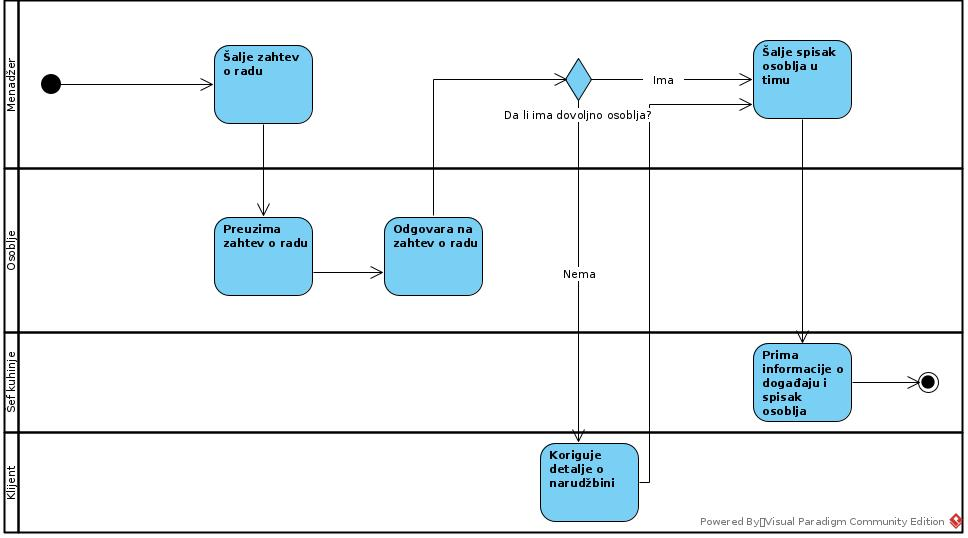
\includegraphics[width=13cm, height=8cm]{Milica/Dijagram_aktivnosti_Formiranje_tima.jpg}
    \caption{Dijagram aktivnosti Formiranje tima za događaj }
    \label{fig:FormiranjeTima}
\end{figure}

\subsubsection{Priprema hrane za događaj}
\begin{itemize}
    \item Kratak opis:
    \begin{itemize}
        \item Šef kuhinje zadaje zadatke za osoblje. Priprema hrane.
    \end{itemize}
\end{itemize}
  \begin{itemize}
        \item Učesnici:
          \begin{itemize}
        \item Šef kuhinje
    \end{itemize}
      \begin{itemize}
        \item Osoblje
    \end{itemize}
    \end{itemize}
      \begin{itemize}
        \item Preduslov:
          \begin{itemize}
        \item Šef kuhinje je obavešten o detaljima narudžbine. Šef kuhinje ima spisak osoblja koji su raspoloživi za događaj.
   \end{itemize}
    
    \end{itemize}
      \begin{itemize}
        \item Postuslov:
          \begin{itemize}
        \item Narudžbina je gotova za dogovoreno vreme.
    \end{itemize}
    \end{itemize}
      \begin{itemize}
        \item Glavni tok:
          \begin{enumerate}
              
        
              \item Šef kuhinje, u zavisnosti od vrste hrane koja je naručena i sposobnostima osoblja, zadaje zadatke osoblju. Svako od osoblja ima na aplikaciji koji je njegov deo posla, kao i koji su delovi posla ostalih članova u timu. 
        
              \item Svako od osoblja procenjuje koliko vremena je potrebno da izvrši zadati posao i  unosi procenjeno vreme u aplikaciju.
         
              \item Šef kuhinje, u zavisnosti od procenjenog vremena osoblja i zakazanog termina događaja, zakazuje početak radnog vremena.
       
              \item Svako od osoblja, u dogovoreno vreme,  počinje sa izvršavanjem svog dela posla i priprema ketering.
          
          \end{enumerate}
    \end{itemize}
      \begin{itemize}
        \item Alternativni tok:
          \begin{itemize}
        \item Korak 3 - Ukoliko procenjeno vreme završavanja posla prekorači zakazano vreme događaja, šef kuhinje pronalazi putem aplikacije potrebno osoblje. Jedan od načina za to je da šef kuhinje šalje zahtev osoblju koje je odbilo zahtev menadžera, a bilo je raspoloživo za datum događaja. Proces se nastavlja u koraku 3.
    \end{itemize}
    \end{itemize}
    
\begin{figure}[H]
    \centering
    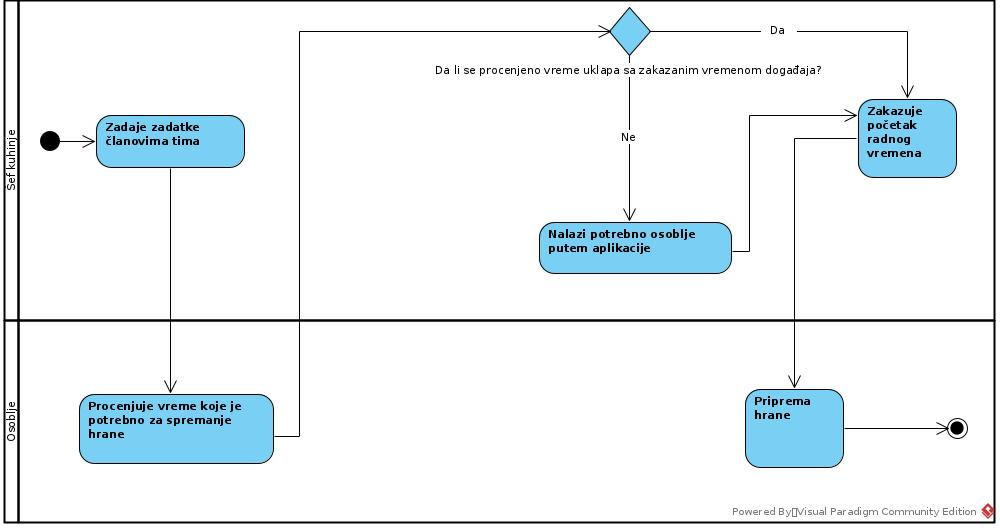
\includegraphics[width=14cm, height=8cm]{Milica/Dijagarm_aktivnosti_Priprema_hrane.jpg}
    \caption{Dijagram aktivnosti Priprema hrane }
    \label{fig:RegistracijaZ}
\end{figure}
    

\subsubsection{Dostava keteringa}
\begin{itemize}
    \item Kratak opis:
    \begin{itemize}
 
        \item Menadžer korišćenjem informacionog sistema obaveštava dostavljača o terminu i lokaciji isporuke poručenog keteringa. Dostavljač potvrđuje dostavu.Dostavljač prevozi u određeno vreme na određenu lokaciju poručeni ketering.
        Klijent preuzima ketering.
    \end{itemize}
    
    
\end{itemize}


  \begin{itemize}
        \item Učesnici:
         \begin{itemize}
        \item Menadžer
    \end{itemize}
          \begin{itemize}
        \item Klijent
    \end{itemize}
      \begin{itemize}
        \item Dostavljač
    \end{itemize}
    \end{itemize}
      \begin{itemize}
        \item Preduslov:
          \begin{itemize}
        \item Osoblje u kuhinji je završilo posao na vreme.
       
   \end{itemize}
    
    \end{itemize}
      \begin{itemize}
        \item Postuslov:
          \begin{itemize}
        \item Porudžbina je dostavljena klijentu za događaj.
    \end{itemize}
    \end{itemize}
      \begin{itemize}
        \item Glavni tok:
          \begin{enumerate}
          
              \item Menadžer šalje zahtev dostavljaču preko aplikacije sa detaljima isporuke.
              
              \item Dostavljač prima zahtev i informacije o dostavi.
          
              \item Dostavljač potvrđuje da li je slobodan da dostavi porudžbinu ili ne.
              
              \item Dostavljač vrši dostavu. Prvo se informiše kako može da dođe na lokaciju događaja, zatim uzima u obzir nepredviđene okolnosti na putu i obračunava vreme polaska shodno tome. Dostavljač procenjuje koliko mu je vremena potrebno da dostavi porudžbinu. U zavisnosti od procenjenog vremena dostavljač određuje vreme polaska, prevozi poručen ketering i stiže u dogovoreno vreme.
         
              \item Klijent preuzima porudžbinu.
          \end{enumerate}
    \end{itemize}
      \begin{itemize}
        \item Alternativni tok:
          \begin{itemize}
        \item Korak 2 - Ukoliko dostavljač da negativan odgovor, menadžer pronalazi drugog dostavljača putem aplikacije. Proces se nastavlja u koraku 2.
    \end{itemize}
    \end{itemize}
    
\begin{figure}[H]
    \centering
    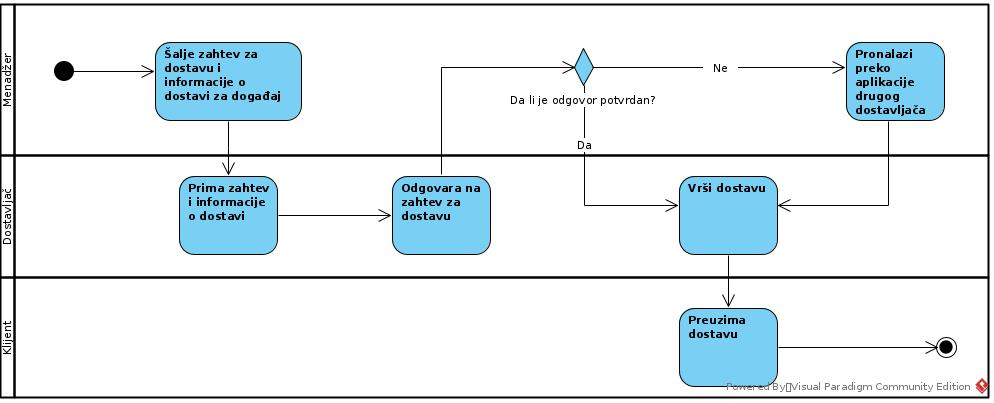
\includegraphics[width=15cm, height=8cm]{Milica/Dijagram_aktivnosti_Dostava_ketering.jpg}
    \caption{Dijagram aktivnosti Dostava keteringa}
    \label{fig:RegistracijaZ}
\end{figure}


%kraj-Milica
%%%%%%%%%%%%%%%%

\subsection{Naplata usluge}

\begin{figure}[H]
    \centering
    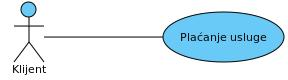
\includegraphics[width=6cm]{Nina/Slucaj_upotrebe_naplata.jpg}
    \caption{Dijagram slučaja upotrebe Naplata usluge}
    \label{fig:RegistracijaZ}
\end{figure}

\begin{itemize}
    \item Kratak opis: 
    \begin{itemize}
        \item Kada je usluga koju je klijent odabrao potpuno završena, on uplaćuje prethodno definisanu svotu novca preko sistema.
    \end{itemize}
    \item Učesnici:
        \begin{itemize}
        \item Klijent
    \end{itemize}
    \item Preduslov:
        \begin{itemize}
            \item Usluga koju je klijent izabrao je potpuno završena.
            \item Klijent ima otvoren nalog za korišćenje sistema.
        \end{itemize}
    \item Postuslov:
        \begin{itemize}
            \item Uplata je uspešno obavljena.
            \end{itemize}
    \item Glavni tok:
        \begin{enumerate}
            \item Klijent se prijavljuje na sistem firme Duma Group.
            \item Klijent klikom na link 'PLATI' dobija formular za izvršavanje naplate
            \item Klijent popunjava formular podacima koji nedostaju kako bi izvršio uplatu korišćene usluge.
            \item Klijent potvrđuje uplatu.
            \item Sistem vrši validaciju uplate.
            \item Sistem beleži uslugu kao uspešno regulisanu i ažurira dugovanje klijenta koje je prikazano na profilu.
        \end{enumerate}
    \item Alternativni tok:
        \begin{itemize}
            \item Korak 5 - Ukoliko uplata nije validna (broj računa je nepostojeći ili nije u dobrom formatu), sistem obaveštava korisnika o grešci i proces se nastavlja u koraku 4.  
    \end{itemize}
    \item Dodatne informacije:
        \begin{itemize}
            \item Cena koju klijent plaća je ažurirana tokom sprovođenja usluge.
            \item Podaci koje klijent treba da popuni su ime, prezime, adresa i broj računa.
        \end{itemize}
\end{itemize}

\begin{figure}[H]
    \centering
    \includegraphics[width=10cm, height=5cm]{Nina/DijagramAktivnostiNaplata.jpg}
    \caption{Dijagram aktivnosti naplate usluge}
    \label{fig:RegistracijaZ}
\end{figure}

\section{Model baze podataka}

Analizom slučajeva upotrebe informacionog sistema firme Duma Group, projektovana je baza podataka. Na slici \ref{fig:dijagramTabela}  se može videti dijagram tabela koji joj odgovara.

\begin{figure}[H]
    \centering
    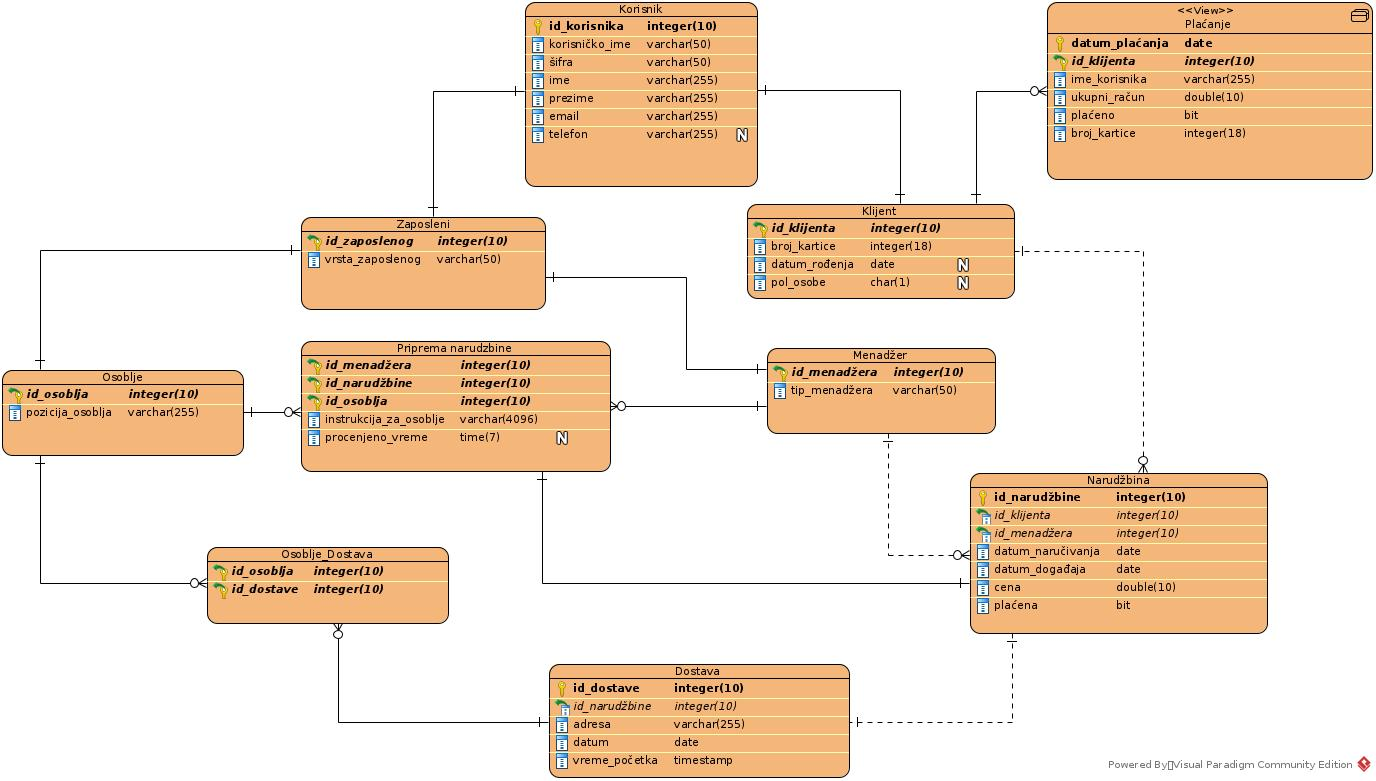
\includegraphics[width=14cm, height=10cm]{baza/dijagram_tabela.jpg}
    \caption{Dijagram tabela baze podataka}
    \label{fig:dijagramTabela}
\end{figure}

\subsection{Nezavisni entiteti}

Nezavisni entitet naše baze podataka je \textbf{Korisnik}. Da bi se korisnik registrovao na sistem potrebna mu je email adresa, a da bi se prijavio potrebno mu je korisničko ime i šifra. Atributi:
\begin{itemize}
    \item id\_korisnika - id korisnika koji predstavlja primarni ključ ovog entiteta
    \item korisničko\_ime - korisničko ime korisnika pomoću kog se prijavljuje na sistem
    \item šifra - enkriptovana šifra korisnika potrebna pri prijavljivanju
    \item ime
    \item prezime
    \item email - email adresa korisnika potrebna pri registrovanju
    \item telefon - može da ostane nepopunjeno
\end{itemize}


\subsection{Izvedeni entiteti}

Izvedeni entiteti naše baze podataka su:
\begin{enumerate}
    \item Klijent
    \item Zaposleni
    \item Menadžer
    \item Osoblje
\end{enumerate}

\vspace{3mm}

\textbf{Klijent} predstavlja specijalizaciju entiteta Korisnik. On predstavlja osobe koje uzimaju usluge firme Duma Group. Atributi:
\begin{itemize}
    \item id\_klijenta - id klijenta koji predstavlja strani ključ ka entitetu Korisnik, a ujedno i primarni ključ ove tabele
    \item broj\_kartice - broj kartice klijenta pomoću kog će izvršiti plaćanje
    \item datum\_rođenja
    \item pol\_osobe
\end{itemize}

\vspace{3mm}

\textbf{Zaposleni} predstavlja specijalizaciju entiteta Korisnik. On predstavlja osobe koje su zaposlene u firmi Duma Group. Atributi:
\begin{itemize}
    \item id\_zaposlenog - id zaposlenog koji predstavlja strani ključ ka entitetu Korisnik, a ujedno i primarni ključ ove tabele
    \item vrsta\_zaposlenog - koja je vrsta zaposlenog u pitanju(Osoblje, Menadžer, Administrator...)
\end{itemize}

\vspace{3mm}

\textbf{Menadžer} predstavlja specijalizaciju entiteta Zaposleni. On predstavlja osobu koja je zadužena za komunikaciju sa klijentom prilikom pravljenja narudžbine i za prenošenje detalja narudžbine osoblju. Atributi:
\begin{itemize}
    \item id\_menadžera - id menadžera koji predstavlja strani ključ ka entitetu Zaposleni, a ujedno i primarni ključ ove tabele
    \item tip\_menadžera - za koju uslugu je ovaj menadžer zadužen(Ketering, Prenosivi bar, Fotografija) 
\end{itemize}

\vspace{3mm}

\textbf{Osoblje} predstavlja specijalizaciju entiteta Zaposleni. Osoblje čine osobe koje rade na samom događaju, kao što su barmeni, fotografi, šef kuhinje i dostavljač. Atributi:
\begin{itemize}
    \item id\_osoblja - id osoblja koji predstavlja strani ključ ka entitetu Zaposleni, a ujedno i primarni ključ ove tabele
    \item pozicija\_osoblja - koji član osoblja je u pitanju(barmen, fotograf, šef kuhinje, dostavljač) 
\end{itemize}


\vspace{3mm}

\subsection{Agregirani entiteti}

Agregirani entiteti naše baze podataka su:
\begin{enumerate}
    \item Narudžbina
    \item Dostava
    \item Priprema narudžbine
    \item Osoblje dostava
\end{enumerate}


\vspace{3mm}

\textbf{Narudžbina} sadrži informacije o narudžbinama, odnosno njenim detaljima. Atributi:
\begin{itemize}
    \item id\_narudžbine - id narudžbine koja je poručena, predstavlja primarni ključ ovog entiteta
    \item id\_menadžera - id menadžera firme, koji predstavlja strani ključ ka entitetu Menadžer
    \item id\_klijenta - id klijenta, koji predstavlja strani ključ ka entitetu Klijent
    \item datum\_naručivanja - datum naručivanja usluge
    \item datum\_događaja - datum za koji je usluga naručena
    \item cena - cena usluge koja je poručena
    \item plaćena - ukazuje da li je plaćena usluga (1 ili 0)
    
\end{itemize}

\vspace{3mm}



\textbf{Dostava} sadrži informacije vezane za dostavu. Atributi:
\begin{itemize}
    \item id\_dostave - id dostave koja je zakazana, predstavlja primarni ključ ovog entiteta
    \item id\_narudžbine - id narudžbine koja je poručena, predstavlja strani ključ ka entitetu Narudžbina
    \item adresa - adresa gde treba dostaviti porudžbinu
    \item datum - datum događaja
    \item vreme\_početka - vreme početka događaja
    
\end{itemize}

\vspace{3mm}

\textbf{Priprema\_narudžbine} sadrži informacije o pripremi narudžbine i njenim detaljima, kao i o posebnim zahtevima korisnika. Atributi:
\begin{itemize}
    \item id\_menadžera - id menadžera firme, koji predstavlja strani ključ ka entitetu Menadžer, a ujedno i deo primarnog ključa ove tabele
    \item id\_narudžbine - id narudžbine koja je poručena, strani ključ ka entitetu Narudžbina, a ujedno i deo primarnog ključa ove tabele
    \item id\_osoblja - id osoblja koje priprema narudžbinu, strani ključ ka entitetu Osoblje, a ujedno i deo primarnog ključa ove tabele
    \item instrukcija\_za\_osoblje - detaljan opis narudžbine i opis zadataka koje osoblje treba da ispuni
    \item procenjeno\_vreme - očekivano vreme za pripremu narudžbine
    
\end{itemize}

\vspace{3mm}

\textbf{Osoblje\_Dostava} povezuje entitete Osoblje i Dostava. Atributi:
\begin{itemize}
    \item id\_dostave - id dostave koja je zakazana, predstavlja strani ključ ka entitetu Dostava i deo primarnog ključa ovog entiteta
    \item id\_osoblja - id osoblja koje vrši dostavu, predstavlja strani ključ ka entitetu Osoblje i deo primarnog ključa za ovaj entitet
    
\end{itemize}

\vspace{3mm}


\subsubsection{Pogledi}

Kako bi se pojednostavilo rukovanje bazom podataka, uveden je i pogled \textbf{Plaćanje}. Ovaj pogled sadrži sve detalje koji su potrebni kako bi klijent obavio plaćanje svog računa. Atributi:
\begin{itemize}
    \item datum\_plaćanja - datum kada je održan događaj za koji se plaća usluga, koji predstavlja deo primarnog ključa ovog pogleda
    \item id\_klijenta - id klijenta koji obavlja plaćanje, koji predstavlja strani ključ ka entitetu Klijent, a ujedno i deo primarnog ključa ovog pogleda
    \item ime\_korisnika 
    \item ukupni\_račun - ukupni račun koji dobijemo kada saberemo cene svega onoga što je klijent naručio
    \item plaćeno - govori nam da li je račun izmiren ili ne (vrednost je 0 ako nije, 1 ako jeste)
    \item broj\_kartice - broj kartice klijenta pomoću kog će izvršiti plaćanje
\end{itemize}

\section{Arhitektura sistema}
U ovom poglavlju će biti predstavljena predložena arhitektura sistema.

\subsection{Karakteristike sistema}
Arhitektura sistema je razmatrana tako da ispuni što više od navedenih uslova:
\begin{itemize}
    \item Dostupnost
    \item Ažurnost
    \item Odziv
    \item Jednostavnost upotrebe
    \item Stabilnost
    \item Bezbednost
\end{itemize}
Odabrana je Veb aplikacija jer pruža visok stepen dostupnosti i ažurnosti, jer izmenom Veb aplikacije svi korisnici sistema automatski dobijaju izmene. Odziv se lako postiže sve dok korisnik ima računar prosečnih performansi i solidnu internet konekciju. Jednostavnost upotrebe se dobija pažljivo dizajniranim korisničkim interfejsom, pri čemu je glavna motivacija da on bude jednostavan i da ne opterećuje korisnika nepotrebnim detaljima pri korišćenju aplikacije. Bezbednost je postignuta troslojnom arhitekturom.

\begin{enumerate}
    \item Tip aplikacije: Veb aplikacija
    \item Strategija isporučivanja: Jedan serverski i više klijentskih računara
    \item Tehnologije: Angular framework, NodeJS, Java, relaciona baza podataka
\end{enumerate}

\subsection{Tip i slojevi sistema}

Za informacioni sistem izabrana je višeslojna komponentna klijent-server arhitektura, koja se sastoji od narednih slojeva:

\begin{itemize}
    \item Prezentacioni sloj
    \item Klijentski kontroler
    \item Serverski kontroler
    \item Sloj podataka
\end{itemize}


\subsubsection{Prezentacioni sloj}

Prezentacioni sloj predstavlja najviši nivo aplikacije i zadužen je da korisniku prikaže sadržaj koji dobija od nižih slojeva arhitekture. Njegov glavni zadatak je da korisniku na što efikasniji i jednostavniji način omogući korišćenje aplikacije.
\newline
Sastoji se iz komponenti:
\begin{itemize}

\item Registrovanje
\item Prijavljivanje
\item Izmena ličnih podataka
\item Odabir ponude

\end{itemize}
\subsubsection{Klijentski kontroler}

Glavni zadatak klijentskog kontrolera je da komunicira sa serverskim slojem sistema. Takođe, zadužen je za prosleđivanje podataka prezentacionom sloju, koji dalje predstavlja podatke korisniku.
\newline
Sastoji se iz komponenti:
\begin{itemize}
\item Validacija
\item Dohvatanje podataka
\item Autorizacija i autentifikacija
\end{itemize}



\subsubsection{Serverski kontroler}

Serverski kontroler ima sličnu svrhu kao klijentski kontroler, s tim što klijent nema pristup ovom delu aplikacije. Ovo je obezbeđeno prvenstveno zbog bezbednosti i kako bi se u ovom delu mogla izvršiti detaljnija autorizacija i validacija podataka. Ovde se takođe vrši i komunikacija sa bazom kao i neophodna izračunavanja nad podacima dobijenim iz baze. 
\newline
Sastoji se iz komponenti:
\begin{itemize}
\item Pregled i izmena ličnih podataka
\item Izračunavanje ukupne cene i naplata
\item Dohvatanje podataka
\item Autorizacija i autentifikacija
\end{itemize}


\subsubsection{Sloj podataka}
Sloj podataka sadrži sve potrebne mehanizme za bezbedno i konzistentno pristupanje bazi podataka. Zadatak ovog sloja je da pruži sve potrebne podatke iz baze uz jednostavan i siguran  pristup.\newline
Sastoji se od komponente:
\begin{itemize}
    \item Baza podataka
\end{itemize}

\begin{figure}[H]
    \centering
    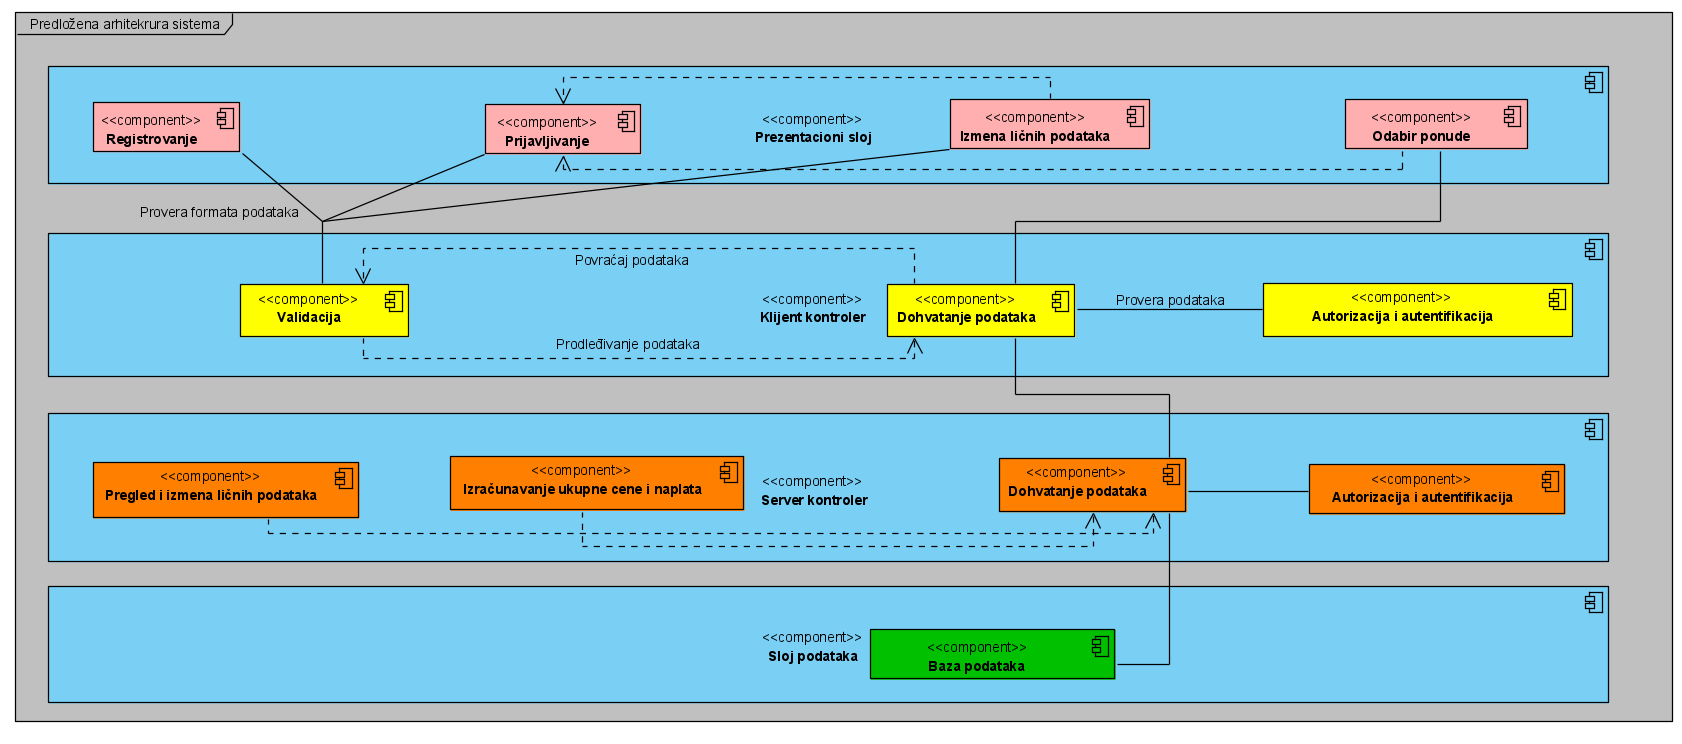
\includegraphics[width=14cm, height=8cm]{Andjela/dijagram_komponenti.png}
    \caption{Dijagram predložene arhitekture sistema}
    \label{fig:dijagramTabela}
\end{figure}

\section{Predlog korisničkog interfejsa}

U ovoj sekciji biće prikazan predlog korisničkog interfejsa sajta firme Duma Group. Sajt koriste klijenti firme.

\subsection{Registracija klijenata}

Na slici \ref{fig:ki_reg} je prikazan način registrovanja klijenata. To je ujedno i početna strana koja se otvara kada se pristupi sajtu firme. Kako bi se registrovao, klijent mora da unese ime, prezime, datum rođenja, pol, korisničko ime, broj kreditne kartice, lozinku, potvrđenu lozinku, email adresu i email za povratak naloga. Registracija se završava klikom na dugme \say{Registruj se}. Ukoliko klijent već ima napravljen nalog, može da klikne na link \say{Prijavi se}, a zatim da se prijavi kao što je objašnjeno u nastavku.

\begin{figure}[H]
    \centering
    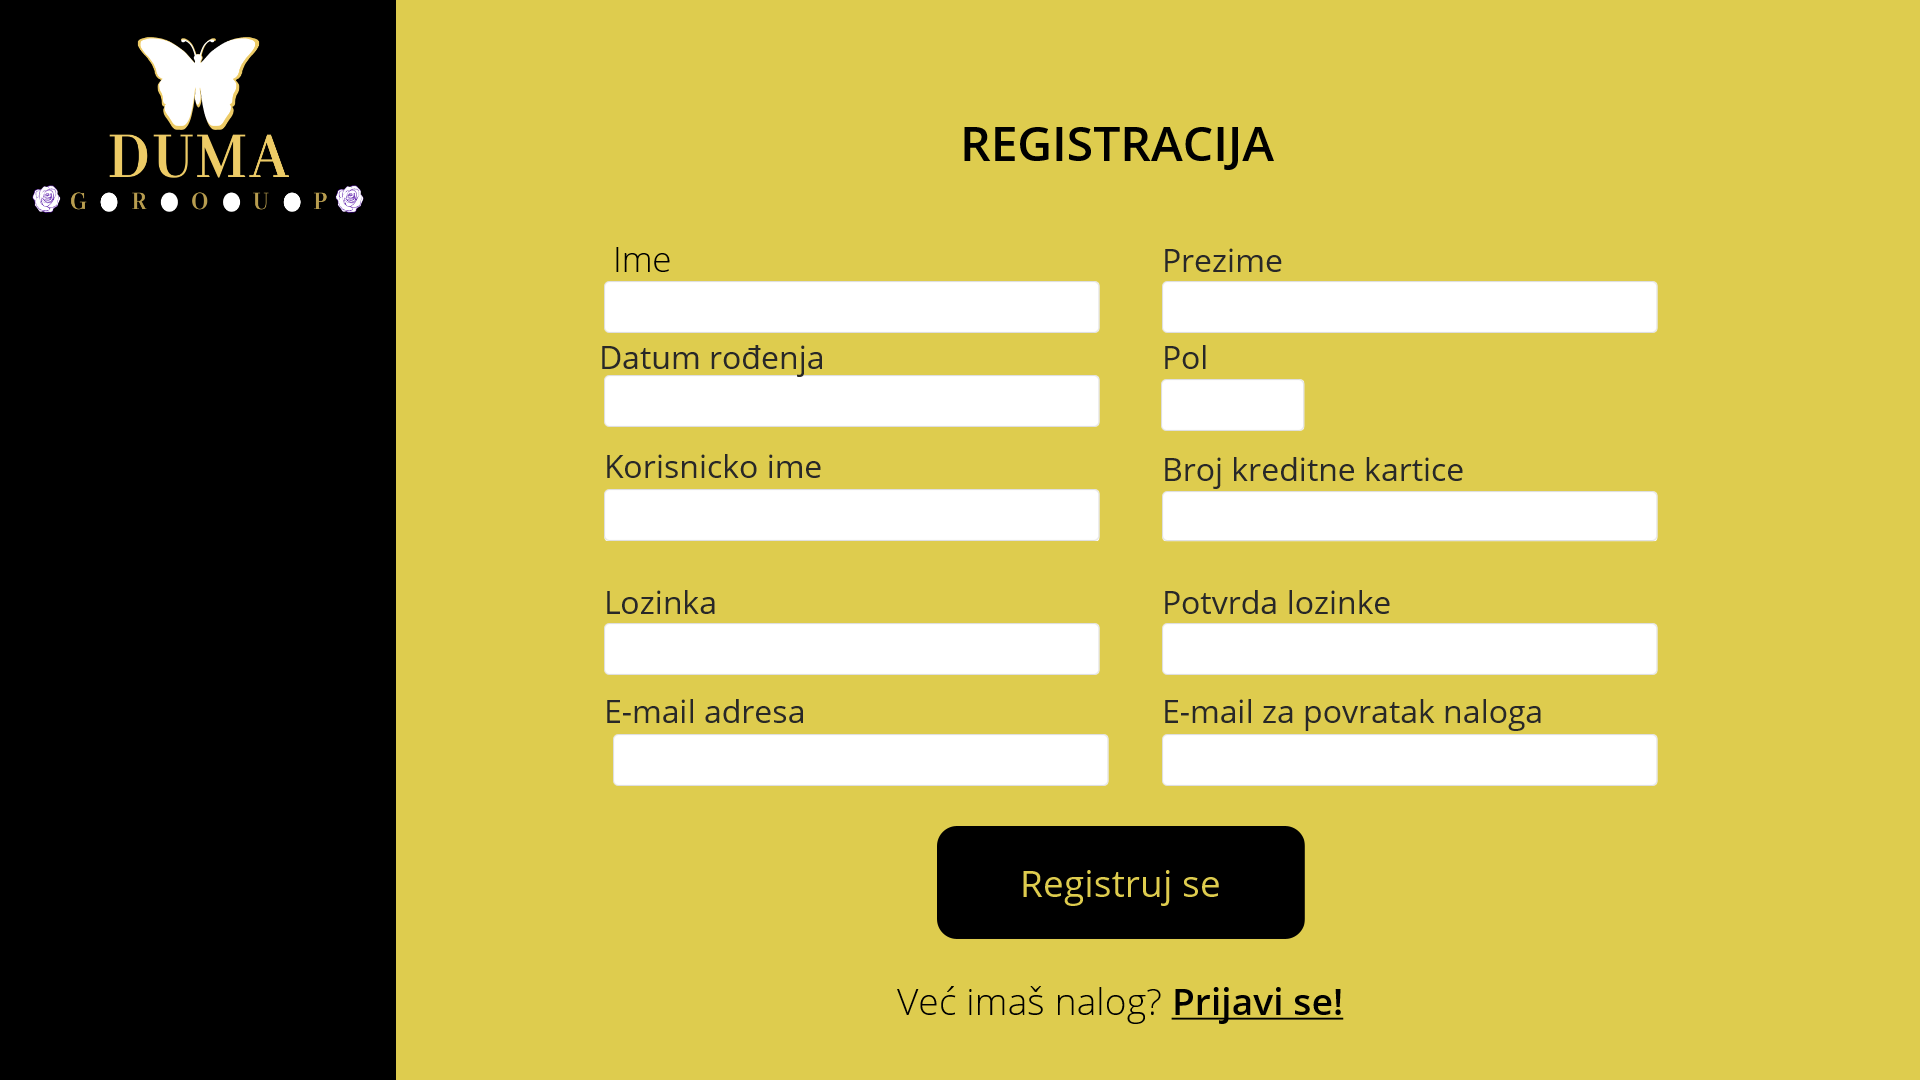
\includegraphics[width=12cm]{interfejs/Registracija.png}
    \caption{Registracija klijenta}
    \label{fig:ki_reg}
\end{figure}

\subsection{Prijava klijenata}

Na slici \ref{fig:ki_prijava} je prikazan način na koji se korisnik prijavljuje. Potrebno je da unese postojeće korisničko ime i lozinku i da klikne na dugme \say{Prijavi se}.

\begin{figure}[H]
    \centering
    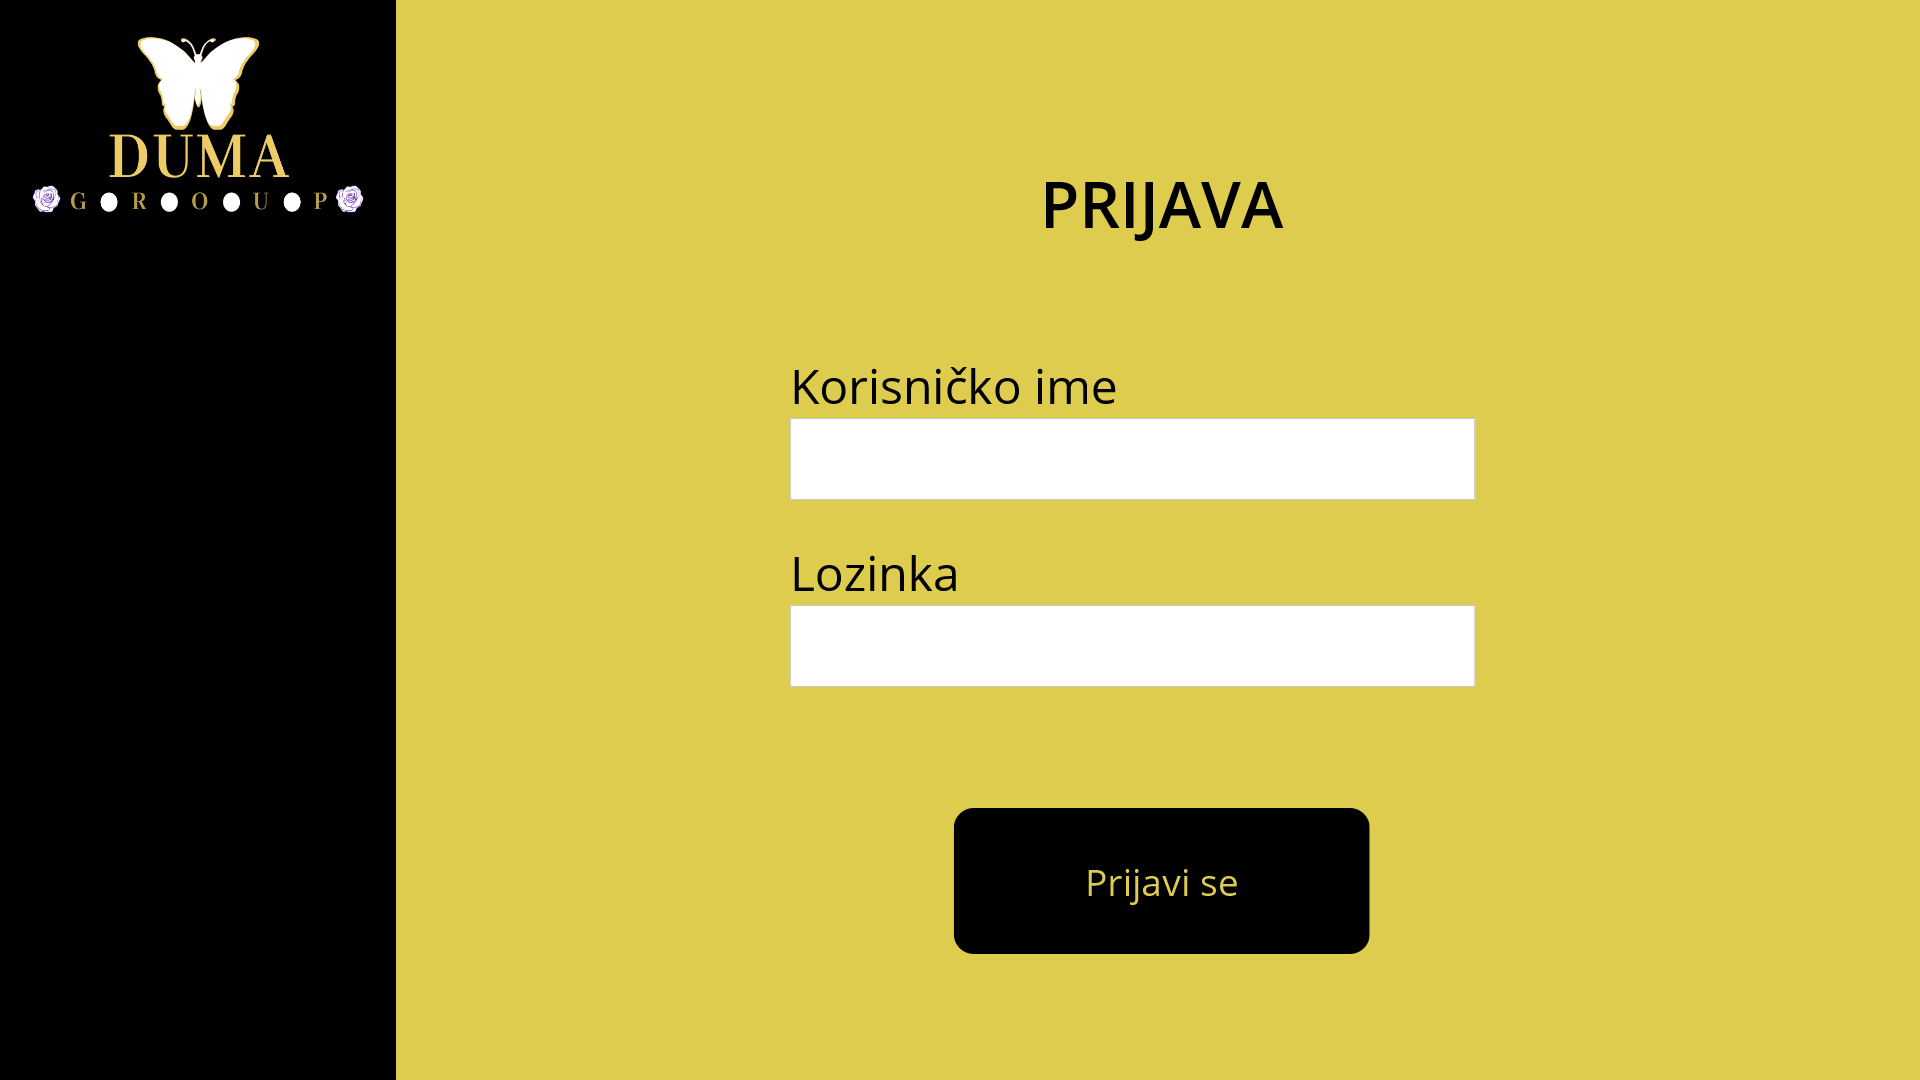
\includegraphics[width=12cm]{interfejs/Prijava.png}
    \caption{Prijava klijenta}
    \label{fig:ki_prijava}
\end{figure}

\subsection{Profil klijenta}

Nakon što se klijent prijavio, na ekranu će mu biti prikazana strana \ref{fig:ki_profil} na kojoj se nalaze informacije o korisniku koje je naveo pri registraciji i slika koju može da promeni. Takođe, klikom na jedno od tri dugmeta, \say{Ketering},  \say{Fotografija} ili \say{Prenosivi bar}, korisnik može da odabere uslugu za koju je zainteresovan. Na profilu se nalazi i ukupno zaduženje za usluge koje je klijent odabrao, kao i link \say{PLATI} ka stranici za izmirivanje tog zaduženja.


\begin{figure}[H]
    \centering
    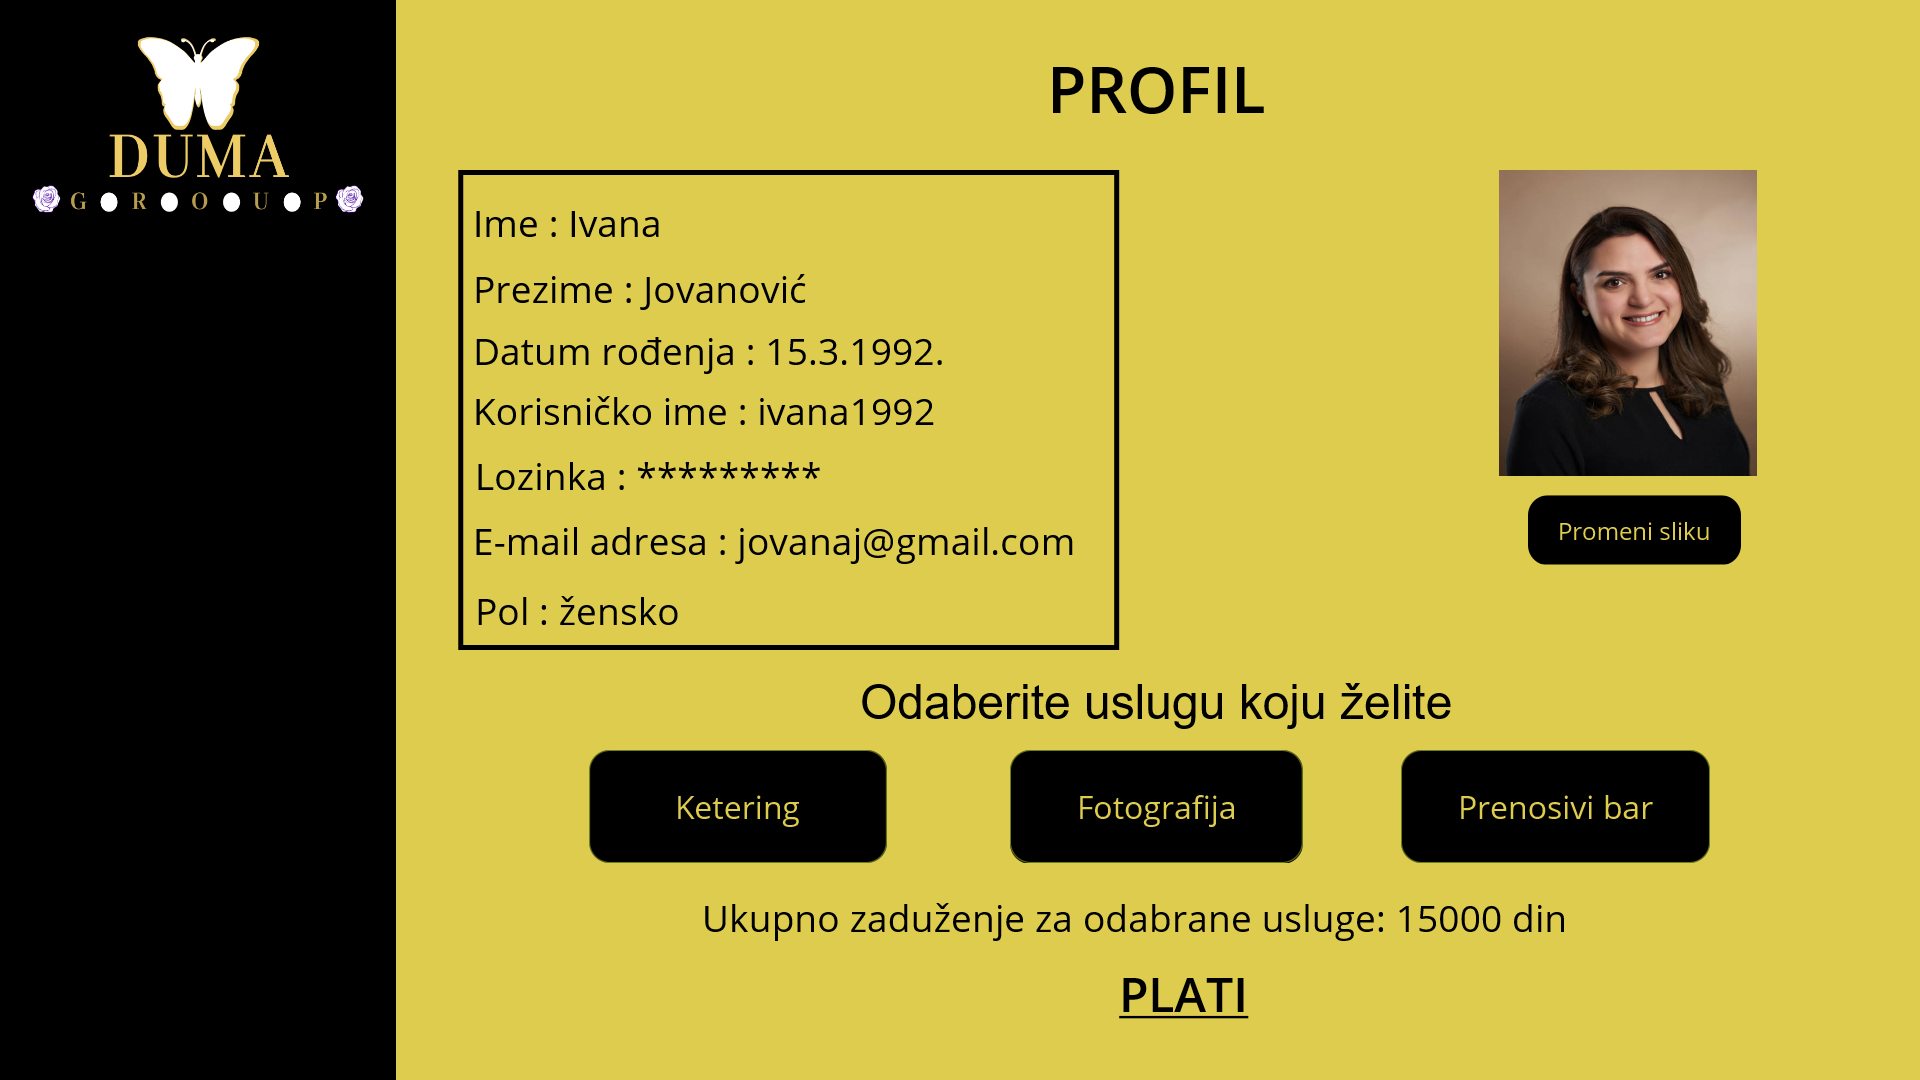
\includegraphics[width=12cm]{interfejs/Profil.png}
    \caption{Profil}
    \label{fig:ki_profil}
\end{figure}

\subsection{Fotografija}

Kao što je već opisano, na profilu korisnik može da izabere jednu od tri usluge koje sistem nudi. Klikom na dugme \say{Fotografija} otvara se formular za naručivanje ove usluge kao na slici \ref{fig:ki_fotografija}. Korisnik treba da popuni polja datum događaja, vreme događaja, mesto događaja, dužina trajanja događaja i da odabere tip fotografisanja koji želi da poruči. Informacije o ceni fotografisanja prikazane su u sekciji za odabir vrste fotografisanja. Proces naručivanja se završava klikom na dugme \say{Naruči}, a cena se dodaje na ukupnu cenu koju korisnik treba da plati i ona je prikazana na profilu korisnika. 

\begin{figure}[H]
    \centering
    
\includegraphics[width=12cm]{interfejs/Fotografija.png}
    \caption{Fotografija}
    \label{fig:ki_fotografija}
\end{figure}

\subsection{Ketering}

Slično kao što je već opisano, pritiskom na dugme \say{Ketering} na profilu, otvara se formular za naručivanje ove usluge, kao što je prikazano na slici \ref{fig:ki_ketering}. Korisnik treba da popuni polja datum događaja, vreme događaja, mesto događaja, broj osoba i da odabere tip keteringa koji želi da poruči. Proces naručivanja se završava klikom na dugme \say{Naruči}, a cena se dodaje na ukupnu cenu koju korisnik treba da plati i ona je prikazana na profilu korisnika.  

\begin{figure}[H]
    \centering
    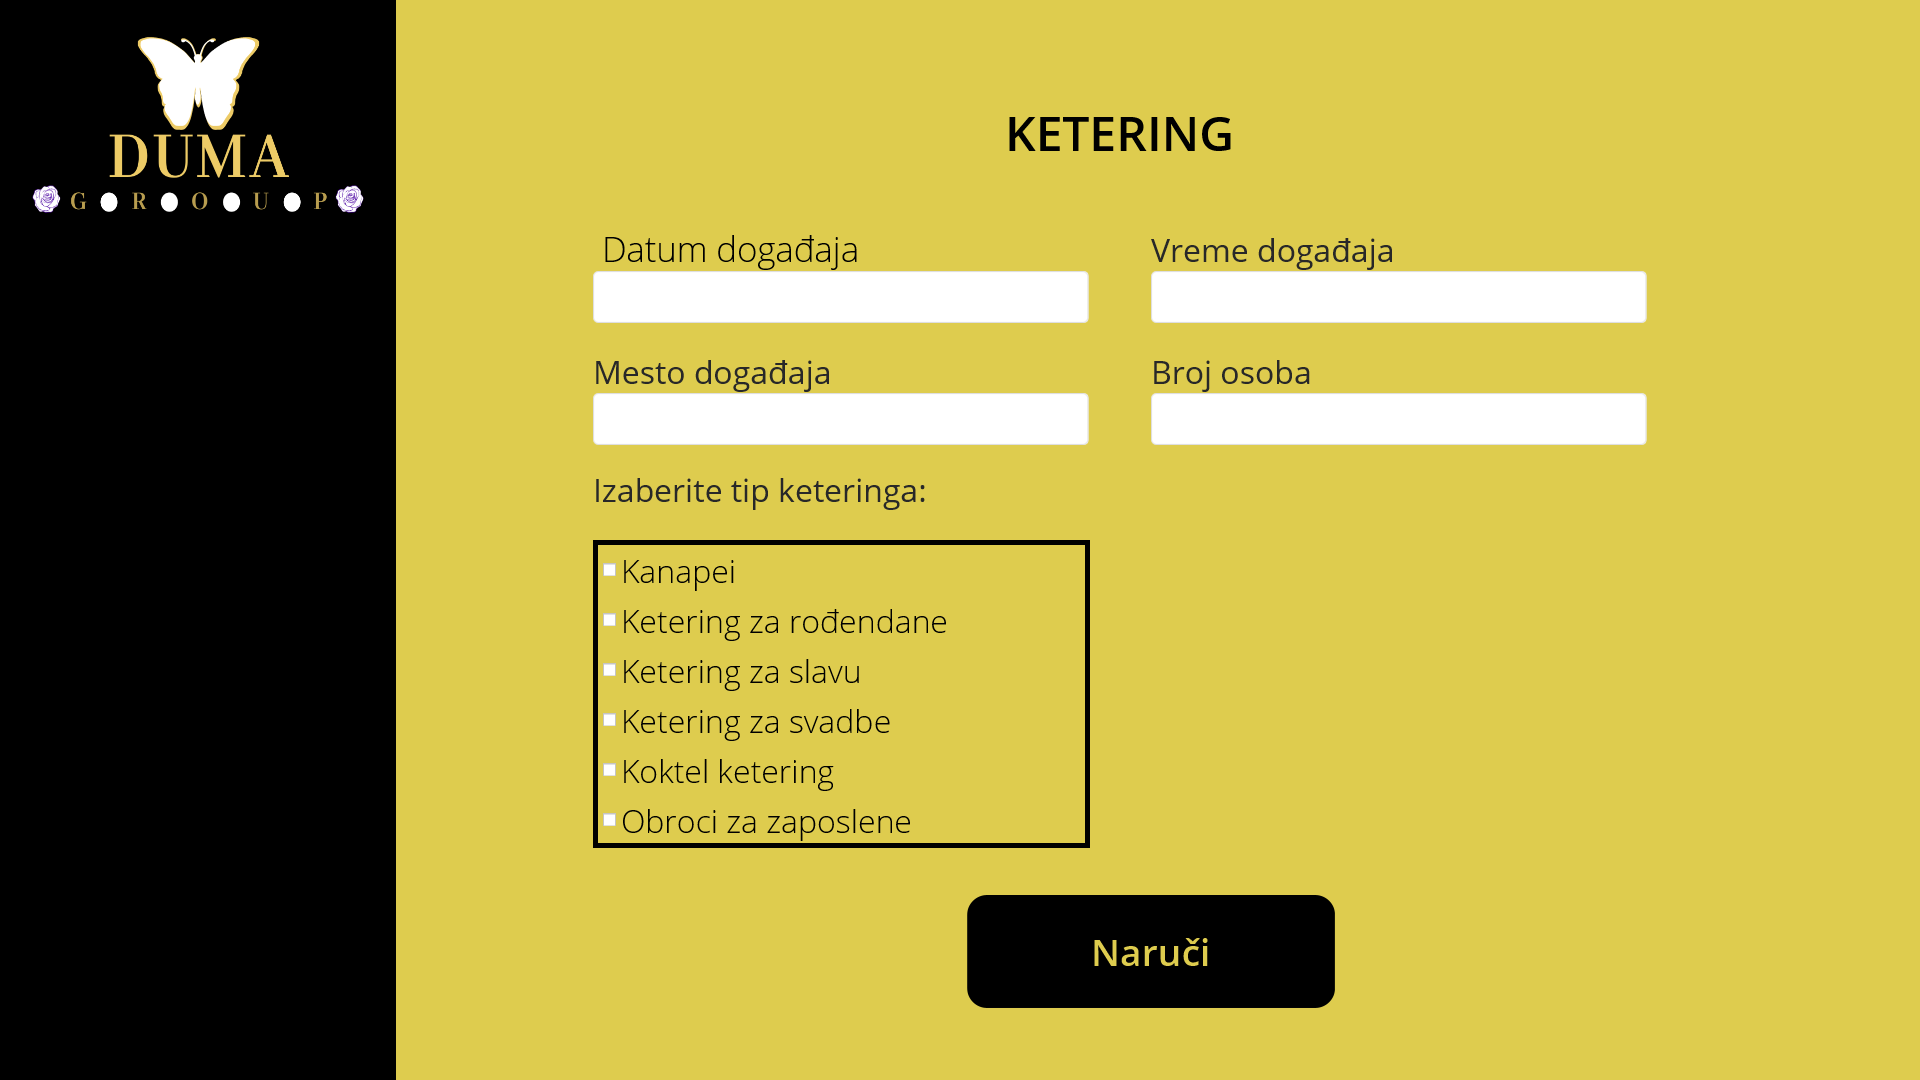
\includegraphics[width=12cm]{interfejs/Ketering.png}
    \caption{Ketering}
    \label{fig:ki_ketering}
\end{figure}

\subsection{Prenosivi bar}

Pritiskom na dugme \say{Prenosivi bar} na profilu, otvara se formular za naručivanje ove usluge, kao što je prikazano na slici \ref{fig:ki_prenosivibar}. Korisnik treba da popuni polja datum događaja, vreme događaja, mesto događaja, dužina trajanja događaja da izabere pića i dekoraciju. Proces naručivanja se završava klikom na dugme \say{Naruči}, a cena se dodaje na ukupnu cenu koju korisnik treba da plati i ona je prikazana na profilu korisnika.  

\begin{figure}[H]
    \centering
    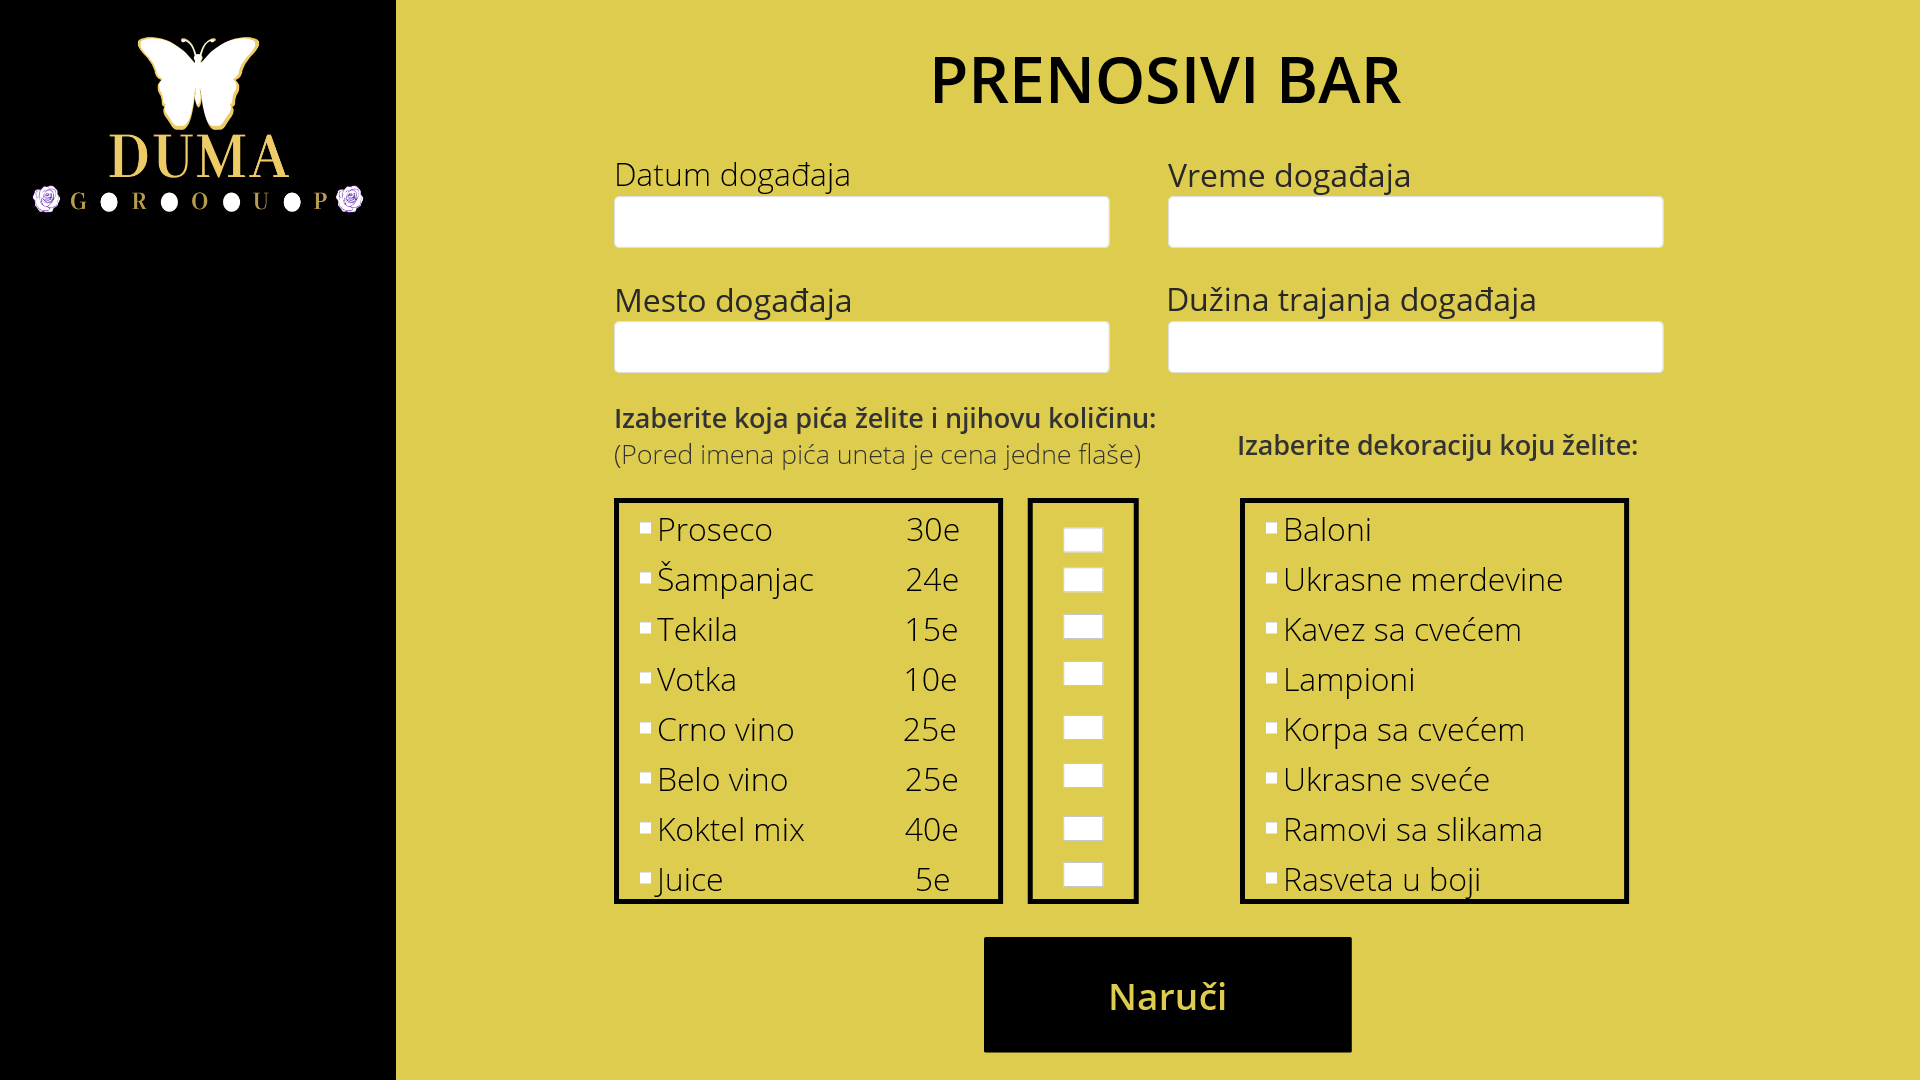
\includegraphics[width=12cm]{interfejs/Prenosivi bar.png}
    \caption{Prenosivi bar}
    \label{fig:ki_prenosivibar}
\end{figure}

\subsection{Plaćanje}

Pritiskom na dugme \say{PLATI} na profilu, otvara se formular za plaćanje usluga, kao što je prikazano na slici \ref{fig:ki_placanje}. Korisnik treba da popuni polja ime, prezime, adresa i broj kreditne kartice. Nakon toga, klikom na dugme \say{Plati}, novac se skida sa njegovog računa, a cena koja se nalazi na njegovom profilu se postavlja na 0e.  

\begin{figure}[H]
    \centering
    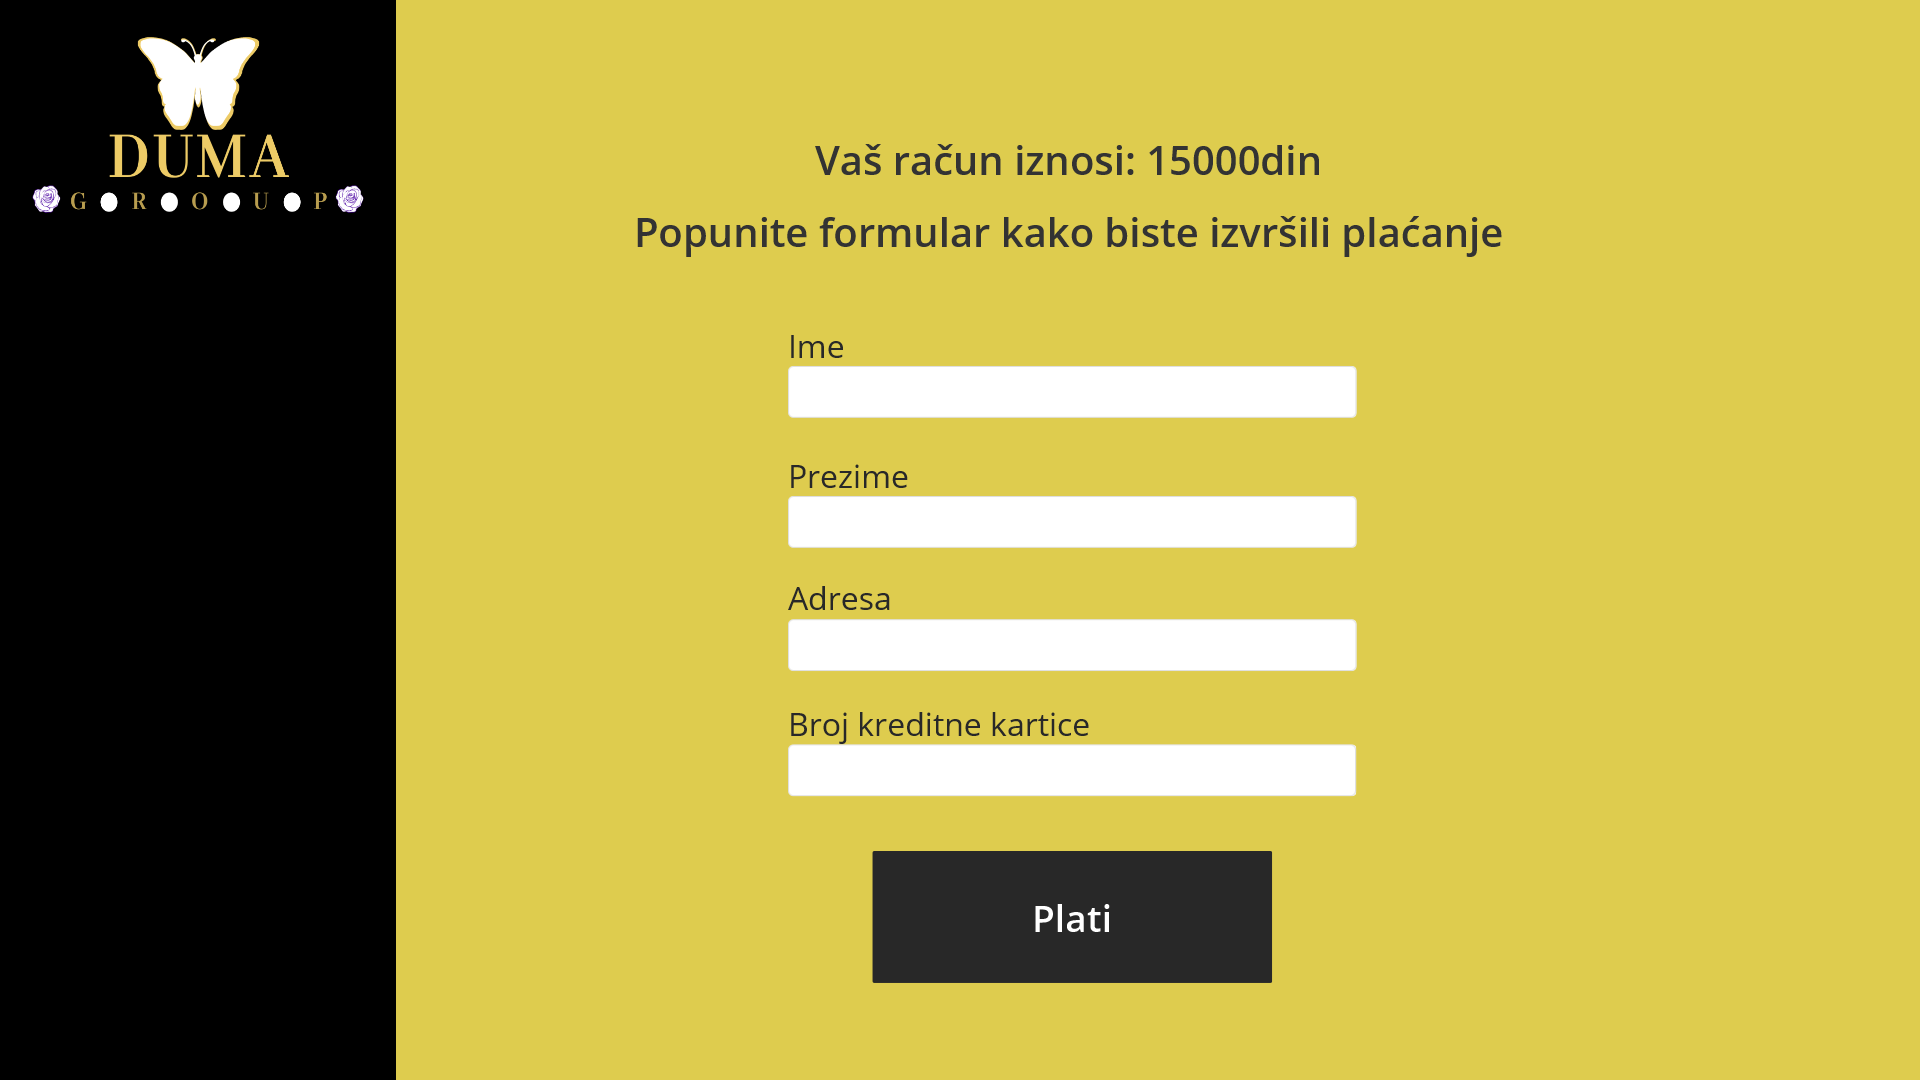
\includegraphics[width=12cm]{interfejs/Placanje.png}
    \caption{Plaćanje}
    \label{fig:ki_placanje}
\end{figure}

\subsection{Potvrda narudžbine}

Nakon što je korisnik popunio formular na strani posvećenoj konkretnoj usluzi, klikom na dugme \say{Naruči} otvara mu se strana kao na slici \ref{fig:ki_kraj}. Ovde korisnik vidi da li je njegova porudžbina uspešno zabeležena. Klikom na dugme \say{Napravi novu porudžbinu} sistem vraća korisnika na profil, gde može da izabere sledeću porudžbinu. Klikom na dugme \say{Odjavi se} sistem vraća korisnika na stranu \say{Prijava} kako bi mogao opet da se prijavi.

\begin{figure}[H]
    \centering
    
\includegraphics[width=12cm]{interfejs/Kraj.png}
    \caption{Potvrda narudžbine}
    \label{fig:ki_kraj}
\end{figure}

\section{Zaključak}

Tokom rada su analizirani i pronađeni nedostaci sistema koji trenutno postoje kod firme Duma Group. Detaljno su opisani slučajevi upotrebe što omogućava razumevanje funkcionisanja jednog ovakvog sistema. Napravljena je šema baze podataka, predložena je arhitektura sistema i neki od procesa su prikazani UML dijagramima. Kreiran je predlog kako bi trebalo da izgleda korisnički interfejs koji koriste klijenti ove firme i prototip koji pruža sliku o potencijalima našeg sistema. Dalji rad bi podrazumevao razvoj samog sistema. 

Rad na projektu se pokazao kao značajan za ceo tim jer smo kroz njega stekli iskustvo rada u timu i znanje koje će nam pomoći, kako u spremanju samog ispita, tako i u radu na nekim narednim projektima. 


\end{document}

